%-%-%-%-%-%-%-%-%-%-%-%-%-%-%-%-%-%-%-%-%-%-%-%-%-%-%-%-%-%-%-%-%-%-%-%-%-%-%
%%% MAIN DOCUMENT %%%

%-%-%-%-%-%-%-%-%-%-%-%-%-%-%-%-%-%-%-%-%-%-%-%-%-%-%-%-%-%-%-%-%-%-%-%-%-%-%

\documentclass[12pt, oneside]{book}
\usepackage{draculatheme}


%%% AESTHETICS %%%
%-%-%-%-%-%-%-%-%-%-%-%-%-%-%-%-%-%-%-%-%-%-%-%-%-%-%-%-%-%-%-%-%-%-%-%-%-%-%


%%% Dimensions and Spacing %%%
\usepackage[margin=1in]{geometry}
\usepackage{setspace}
\linespread{1}
\usepackage{listings}

%%% Define new colors %%%
\usepackage{xcolor}
\definecolor{orangehdx}{rgb}{0.96, 0.51, 0.16}

% Normal colors
\definecolor{xred}{HTML}{BD4242}
\definecolor{xblue}{HTML}{4268BD}
\definecolor{xgreen}{HTML}{52B256}
\definecolor{xpurple}{HTML}{7F52B2}
\definecolor{xorange}{HTML}{FD9337}
\definecolor{xdotted}{HTML}{999999}
\definecolor{xgray}{HTML}{777777}
\definecolor{xcyan}{HTML}{80F5DC}
\definecolor{xpink}{HTML}{F690EA}
\definecolor{xgrayblue}{HTML}{49B095}
\definecolor{xgraycyan}{HTML}{5AA1B9}

% Dark colors
\colorlet{xdarkred}{red!85!black}
\colorlet{xdarkblue}{xblue!85!black}
\colorlet{xdarkgreen}{xgreen!85!black}
\colorlet{xdarkpurple}{xpurple!85!black}
\colorlet{xdarkorange}{xorange!85!black}
\definecolor{xdarkcyan}{HTML}{008B8B}
\colorlet{xdarkgray}{xgray!85!black}

% Very dark colors
\colorlet{xverydarkblue}{xblue!50!black}

% Document-specific colors
\colorlet{normaltextcolor}{black}
\colorlet{figtextcolor}{xblue}

% Enumerated colors
\colorlet{xcol0}{black}
\colorlet{xcol1}{xred}
\colorlet{xcol2}{xblue}
\colorlet{xcol3}{xgreen}
\colorlet{xcol4}{xpurple}
\colorlet{xcol5}{xorange}
\colorlet{xcol6}{xcyan}
\colorlet{xcol7}{xpink!75!black}

% Blue-Purple (should just used colorbrewer...)
\definecolor{xrainbow0}{HTML}{e41a1c}
\definecolor{xrainbow1}{HTML}{a24057}
\definecolor{xrainbow2}{HTML}{606692}
\definecolor{xrainbow3}{HTML}{3a85a8}
\definecolor{xrainbow4}{HTML}{42977e}
\definecolor{xrainbow5}{HTML}{4aaa54}
\definecolor{xrainbow6}{HTML}{629363}
\definecolor{xrainbow7}{HTML}{7e6e85}
\definecolor{xrainbow8}{HTML}{9c509b}
\definecolor{xrainbow9}{HTML}{c4625d}
\definecolor{xrainbow10}{HTML}{eb751f}
\definecolor{xrainbow11}{HTML}{ff9709}

%------- %
% XHFILL %
%------- %


%%% Chapter Headings %%%

% \usepackage[explicit]{titlesec}
% \newcommand*\chapterlabel{}
% \titleformat{\chapter}
%   {\gdef\chapterlabel{}
%    \normalfont\sffamily\Huge\bfseries\scshape}
%   {\gdef\chapterlabel{\thechapter\ }}{0pt}
%   {\begin{tikzpicture}[remember picture,overlay]
%     \node[yshift=-3cm] at (current page.north west)
%       {\begin{tikzpicture}[remember picture, overlay]
%         \draw[fill=LightSkyBlue] (0,0) rectangle
%           (\paperwidth,3cm);
%         \node[anchor=east,xshift=.9\paperwidth,rectangle,
%               enhanced,
% sharp corners=20pt,inner sep=11pt,
%               fill=MidnightBlue]
%               {\color{white}\chapterlabel#1};
%        \end{tikzpicture}
%       };
%    \end{tikzpicture}
%   }
% \titlespacing*{\chapter}{0pt}{50pt}{-60pt}

% \usepackage[Conny]{fncychap}
% \usepackage[Rejne]{fncychap}
% \ChNameVar{\bfseries}  % Makes the chapter "Chapter #" bold
% \ChNumVar{\bfseries}   % Makes the chapter number bold
% \ChTitleVar{\bfseries} % Makes the chapter title bold
% % Define a custom color, for example:
% \definecolor{mycolor}{RGB}{0,128,255}

% % Redefine the chapter style in Rejne to change the line colors
% \makeatletter
% \ChRuleWidth{2pt}   % Change the thickness of the lines
% \renewcommand{\DOCH}{%
%   \vspace*{-50\p@}% Moves the chapter title up/down if needed
%   {\color{mycolor} \hrule \@chapapp{} \space \thechapter \hrule}% Customizes the chapter header with color
% }
% \renewcommand{\DOTI}[1]{%
%   \vskip 20\p@ % Adjusts the space above the title
%   \bfseries #1\par % Embolden the title
%   \vskip 20\p@ % Adjusts the space below the title
% }
% \makeatother

% %% Change Chapter Heading Placement %%
% \usepackage{etoolbox}
% \makeatletter
% \patchcmd{\@makechapterhead}{\vspace*{50\p@}}{\vspace*{-20\p@}}{}{}
% \patchcmd{\@makeschapterhead}{\vspace*{50\p@}}{\vspace*{-20\p@}}{}{}
% \patchcmd{\DOTI}{\vskip 80\p@}{\vskip 40\p@}{}{}
% \patchcmd{\DOTIS}{\vskip 40\p@}{\vskip 0\p@}{}{}
% \makeatother

\renewcommand{\thesection}{\thechapter.\arabic{section}} %% Chapter.Section Numbering


%%% FIGURES %%%
\usepackage{graphicx}  
\graphicspath{ {images/} }  
% \numberwithin{figure}{section}
\usepackage{float}
\usepackage{caption}

%%% Hyperlinks %%%
\usepackage{hyperref}
\definecolor{horange}{HTML}{f58026}
\hypersetup{
	colorlinks=true,
	linkcolor=horange,
	filecolor=horange,      
	urlcolor=horange,
}


%% Headers and Footers %%
\usepackage{fancyhdr} % This should be set AFTER setting up the page geometry
\pagestyle{fancy} % options: empty , plain , fancy
\renewcommand{\chaptermark}[1]{\markboth{\thechapter.\ #1}{}}
\fancyhead[R]{\leftmark}
\fancyhead[L]{Hendrix College}
\fancyhead[C]{
\includegraphics[height=.50cm]{images/small logo.png}}
\usepackage{xpatch}
\xpretocmd\headrule{\color{orangehdx}}{}{\PatchFailed}
\setlength{\footskip}{0.5in}
\setlength{\headheight}{18.5764pt}


%%%%% Colored Boxes %%%%%
\usepackage{tcolorbox}
\tcbuselibrary{skins}
\tcbuselibrary{theorems}
\tcbuselibrary{minted}
\newcounter{BoxCounter}


\newtcolorbox{note}{colback=black!15!white, colframe=black, boxrule=0.5mm, arc=4mm, left=4mm, right=4mm, top=2mm, bottom=2mm}

%% Numbered Theorems %%
\newtcolorbox[use counter=BoxCounter, number within=section]{theorem}[1][]{%
    enhanced,
sharp corners,
    colframe=xblue, %color of frame
    colback=xblue!15, %color of background
    coltitle=white, %color of title text
    label={thm:\theBoxCounter},
    title={\large \textbf{Theorem \theBoxCounter}},
    attach boxed title to top left={xshift=0.5cm},
    boxed title style={colback=xblue},
    #1
}


%% Named Theorems %%
\newtcolorbox[use counter=BoxCounter, number within=section]{ntheorem}[2][]{%
    enhanced,
sharp corners=south,
    colframe=xblue, %color of frame
    colback=xblue!15, %color of background
    coltitle=white, %color of title text
    label={thm:#2},
    title={\large \textbf{Theorem \theBoxCounter: #2}},
    attach boxed title to top center,
    boxed title style={colback=xblue},
    #1
}


%% Definitions %%
\newtcolorbox[use counter=BoxCounter, number within=section]{definition}[2][]{%
    enhanced,
sharp corners=downhill,
    colframe=xred,
    colback=xred!15,
    coltitle=white,
    label={def:#2},
    title={\large \textbf{Definition \theBoxCounter: #2}},
    attach boxed title to top right={xshift=-0.5cm},
    boxed title style={colback=xred},
    #1
}


%% Axioms %%
\newtcolorbox[use counter=BoxCounter, number within=section]{axiom}[2][]{%
    enhanced,
sharp corners=south,
    colframe=xdarkgreen,
    colback=xdarkgreen!15,
    coltitle=white,
    label={ax:#2},
    label={ax:\theBoxCounter},
    title={\large \textbf{Axiom \theBoxCounter: #2}},
    attach boxed title to top center,
    boxed title style={colback=xdarkgreen},
    #1
}


%% Exercises %%
\newcounter{exerciseCounter}

\newtcolorbox[use counter=exerciseCounter]{exercise}[2][]{%
    enhanced,
sharp corners=uphill,
    colframe=orangehdx!75,
    colback=orangehdx!10,
    coltitle=white,
    label={ex:\theexerciseCounter},
    title={\large \textbf{Exercise \theexerciseCounter: #2}},
    attach boxed title to top left={xshift=0.5cm},
    boxed title style={colback=orangehdx!75},
    #1,
}


%% Examples %%
\newcounter{ExampleCounter}
\newtcolorbox[use counter=ExampleCounter, number within=section]{example}[1][]{%
    enhanced,
    sharp corners=south,
    colframe=teal,
    colback=teal!15,
    coltitle=white,
    label={ex:\theExampleCounter},
    title={\large \textbf{Example \theExampleCounter}},
    attach boxed title to top center,
    boxed title style={colback=teal},
    #1,
}


%% Corollaries %%
\newtcolorbox[]{corollary}[3][]{%
    enhanced,
sharp corners,
    colframe=xgrayblue,  
    colback=xgrayblue!15,        
    coltitle=white,
    title={\large \textbf{Corollary to #3: #2}},
    attach boxed title to top left={xshift=0.5cm},
    boxed title style={colback=xgrayblue},
    #1
}


%% Lemmas %%
\newtcolorbox[use counter=BoxCounter, number within=section]{lemma}[1][]{%
    enhanced,
sharp corners=uphill,
    colframe=xpurple,
    colback=xpurple!15,
    coltitle=white,
    label={lm:\theBoxCounter},
    title={\large \textbf{Lemma \theBoxCounter}},
    attach boxed title to top left={xshift=0.5cm},
    boxed title style={colback=xpurple},
    #1,
}

%% Referencing Macros %%

% Exercises
\newcommand{\refex}[1]{\hyperref[ex:#1]{Exercise #1}}

% Definitions
\newcommand{\defword}[2]{\hyperref[def:#2]{#1}}
\newcommand{\defref}[1]{\hyperref[def:#1]{definition of #1}}

% Theorems
\newcommand{\numrefthm}[1]{\hyperref[thm:#1]{Theorem #1}}
\newcommand{\namrefthm}[1]{\hyperref[thm:#1]{#1 Theorem}}

% Axioms
\newcommand{\refax}[1]{\hyperref[ax:#1]{#1 Axiom}}



%-%-%-%-%-%-%-%-%-%-%-%-%-%-%-%-%-%-%-%-%-%-%-%-%-%-%-%-%-%-%-%-%-%-%-%-%-%-%

%% MATH PACKAGES, ENVIRONMENTS, COMMANDS %%
%-%-%-%-%-%-%-%-%-%-%-%-%-%-%-%-%-%-%-%-%-%-%-%-%-%-%-%-%-%-%-%-%-%-%-%-%-%-%
%You'll need your own packages, theorem types, and commands.

\usepackage{fix-cm}
\usepackage{tikz}
\usetikzlibrary{shapes,backgrounds,calc,patterns}
\usepackage{amsmath,amsthm} 
\usepackage{mathtools}
\usepackage{amssymb}
\usepackage{mdframed}
\usepackage{mathrsfs}
\usepackage{changepage}
\usepackage{multicol}
\usepackage{slashed}
\usepackage{enumerate}
\usepackage{booktabs}
\usepackage{pgfplots}
\usepackage{enumitem}
\usepackage{lipsum}  %This package lets us generate random text for example purposes.


%%% Custom Comands %%%
% Natural Numbers 
\newcommand{\N}{\ensuremath{\mathbb{N}}}

% Whole Numbers
\newcommand{\W}{\ensuremath{\mathbb{W}}}

% Integers
\newcommand{\Z}{\ensuremath{\mathbb{Z}}}

% Rational Numbers
\newcommand{\Q}{\ensuremath{\mathbb{Q}}}

% Real Numbers
\newcommand{\R}{\ensuremath{\mathbb{R}}}

% Complex Numbers
\newcommand{\C}{\ensuremath{\mathbb{C}}}

\newcommand{\I}{\ensuremath{\mathbb{I}}}

\newcommand{\pfs}{\noindent\makebox[\linewidth]{\rule{\textwidth}{0.4pt}}\vspace{0.5cm}}

\newcommand{\ale}{\aleph_0}

% \newcommand{}{\marginnote{
\includegraphics[width=2em]{./Math/Intro_to_Adv_Math/images/caution.png}}}

\newmdenv[
  topline=false,
  bottomline=true,
  rightline=false,
  leftline=true,
  linewidth=1.5pt,
  linecolor=black, % default color, will be overridden in custom commands
  backgroundcolor=draculabg, % Needed for Dracula theme
  fontcolor=draculafg, % Needed for Dracula theme
  innertopmargin=0pt,
  innerbottommargin=5pt,
  innerrightmargin=10pt,
  innerleftmargin=10pt,
  leftmargin=0pt,
  rightmargin=0pt,
  skipabove=\topsep,
  skipbelow=\topsep,
]{customframedproof}

\newenvironment{proofpart}[2][black]{
    \begin{mdframed}[
        topline=false,
        bottomline=false,
        rightline=false,
        leftline=true,
        linewidth=1pt,
        linecolor=#1!40, % Custom color
        innertopmargin=10pt,
        innerbottommargin=10pt,
        innerleftmargin=10pt,
        innerrightmargin=10pt,
        leftmargin=0pt,
        rightmargin=0pt,
        skipabove=\topsep,
        skipbelow=\topsep%
    ]
    \noindent
    \begin{minipage}[t]{0.08\textwidth}%
        \textbf{#2}%
    \end{minipage}%
    \begin{minipage}[t]{0.90\textwidth}%
        \begin{adjustwidth}{0pt}{0pt}%
}{
    \end{adjustwidth}
    \end{minipage}
    \end{mdframed}
}


\newcommand{\sbseteqpf}[5][We need to show these expressions are subsets of each other in order to prove they are equivalent.]{%
    \begin{customframedproof}[linecolor=#5]
        \begin{proof}
                #1
            \begin{proofpart}[#5]{(\(\subseteq\))}
                #2
            \end{proofpart}
    \vspace{2mm}
            \begin{proofpart}[#5]{(\(\supseteq\))}
                #3
            \end{proofpart}
    \vspace{2mm}
            #4
        \end{proof}
    \end{customframedproof}
}

% \newcommand{\iffpf}[4]{
%     \begin{customframedproof}[linecolor=#4]
%         \begin{proof}
%             We show this by proving both implications:
%             \begin{proofpart}[#4]{(\(\Rightarrow\))}
%                 #1
%             \end{proofpart}
%     \vspace{2mm}
%             \begin{proofpart}[#4]{(\(\Leftarrow\))}
%                 #2
%             \end{proofpart}
%     \vspace{2mm}
%             #3
%         \end{proof}
%     \end{customframedproof}
% }

\newcommand{\iffpf}[5][We show this by proving both implications:]{
    \begin{customframedproof}[linecolor=#5]
        \begin{proof}
            #1 % This is the optional text, with a default value
            \begin{proofpart}[#5]{(\(\Rightarrow\))}
                #2
            \end{proofpart}
    \vspace{2mm}
            \begin{proofpart}[#5]{(\(\Leftarrow\))}
                #3
            \end{proofpart}
    \vspace{2mm}
            #4
        \end{proof}
    \end{customframedproof}
}



% Command for exercise proofs with a predefined color
\newcommand{\expf}[1]{
    \begin{customframedproof}[linecolor=orangehdx!75,]
        \begin{proof}
        #1
        \end{proof}
    \end{customframedproof}
}

% Command for proofs that are contained within solution environments. 
\newcommand{\innerpf}[1]{%
    \begin{customframedproof}[linecolor=xgray]
        \begin{proof}
            #1
        \end{proof}
    \end{customframedproof}
}


% Command for theorems proofs with a predefined color
\newcommand{\tpf}[1]{
    \begin{customframedproof}[linecolor=xblue]
        \begin{proof}
        #1
        \end{proof}
    \end{customframedproof}
}
% Command for corollaries proofs with a predefined color
\newcommand{\cpf}[1]{
    \begin{customframedproof}[linecolor=purplehdx]
        \begin{proof}
        #1
        \end{proof}
    \end{customframedproof}
}

% Command for the solution environment. Specifically for non-examples. Only for exercises.
\newcommand{\sol}[1]{
    \begin{customframedproof}[linecolor=orangehdx!75,]
        \begin{solution}
        #1
        \end{solution}
    \end{customframedproof}
}

% Command for the solution environment. Specifically for examples.
\newcommand{\lesol}[1]{
    \begin{customframedproof}[linecolor=teal]
        \begin{solution}
        #1
        \end{solution}
    \end{customframedproof}
}

% Command for example proofs. Specifically for examples.
\newcommand{\lepf}[1]{
    \begin{customframedproof}[linecolor=teal]
        \begin{proof}
        #1
        \end{proof}
    \end{customframedproof}
}

\newcommand{\pb}[2]{
    \begin{exercise}
    {#1}#2
    \end{exercise}
}

\def\proofDistance{10pt}
\newenvironment{solution}
  {\textit{Solution.}}

% Command for theorems proofs with a predefined color
\newcommand{\epf}[1]{
    \begin{customframedproof}[linecolor=teal]
        \begin{proof}
        #1
        \end{proof}
    \end{customframedproof}
}

\newcommand{\disabs}[1]{\ensuremath{\left|#1\right|}}
\newcommand{\limn}[1]{\ensuremath{\lim_{n \rightarrow \infty}}#1}

\renewcommand{\theenumi}{\alph{enumi}} 
\renewcommand{\labelenumi}{(\theenumi)}


% end of preamble
%-%-%-%-%-%-%-%-%-%-%-%-%-%-%-%-%-%-%-%-%-%-%-%-%-%-%-%-%-%-%-%-%-%-%-%-%-%-%

\begin{document}

\numberwithin{BoxCounter}{section}


%-%-%-%-%-%-%-%-%-%-%-%-%-%-%-%-%-%-%-%-%-%-%-%-%-%-%-%-%-%-%-%-%-%-%-%-%-%-%
%%% COVER PAGE %%%
%-%-%-%-%-%-%-%-%-%-%-%-%-%-%-%-%-%-%-%-%-%-%-%-%-%-%-%-%-%-%-%-%-%-%-%-%-%-%

% Do not use all caps.
\newcommand{\titlestandin}[0]{Introduction to Advanced Mathematics}
\newcommand{\cussubtitle}[0]{MATH 290}
% Date format should be like: "January 1, 2001"
\newcommand{\startdate}[0]{January 17, 2024}
\newcommand{\customenddate}[0]{May 2, 2024}
% Be sure to include degree recognition (e.g., B.S., M.S., Ph.D)
\newcommand{\professor}[0]{Prof. Carol Ann Downes, Ph.D.}

%-%-%-%-%-%-%-%-%-%-%-%-%-%-%-%-%-%-%-%-%-%-%-%-%-%-%-%-%



\begin{titlepage}
    \begin{center}

        \vspace*{-2cm}
        
\includegraphics[width=0.8\textwidth]{images/Hendrix Logo.png}\\
        \vfill

        % Horizontal line above the title in 'horange' color
        \textcolor{horange}{\rule{\textwidth}{1.0pt}}

        \vspace{2em}

        {\huge \textbf{\titlestandin}}

        \vspace{1em} % Space between the title and the bottom line

        \textcolor{horange}{\rule{\textwidth}{1.0pt}}

        \vspace*{1\baselineskip}

        {\LARGE \textbf{\cussubtitle}}

        \begin{large}
            \vspace*{2\baselineskip}

            \textit{Start}  \\[1ex]
            {\scshape \startdate} \\[0.3\baselineskip] % Year published

            \vspace*{1\baselineskip}

            \emph{Author} \\[1ex]
            %Submitted by \\[\baselineskip]
            {\Large Paul Beggs \\ \par} % Editor list
            {\href{mailto:BeggsPA@Hendrix.edu}{{BeggsPA@Hendrix.edu}}}\\ % Editor affiliation

            \vspace*{1\baselineskip}

            \textit{Instructor} \\[1ex] % Tagline(s) or further description
            \professor

            \vspace*{1\baselineskip}

            \textit{End}\\[1ex]
            {\scshape  \customenddate} \\[0.3\baselineskip] % Year published

            \thispagestyle{empty}

        \end{large}
    \end{center}
\end{titlepage}
\pagebreak


%-%-%-%-%-%-%-%-%-%-%-%-%-%-%-%-%-%-%-%-%-%-%-%-%-%-%-%-%-%-%-%-%-%-%-%-%-%-%

%%% Table of Contents %%%

% No need to edit.

% -%-%-%-%-%-%-%-%-%-%-%-%-%-%-%-%-%-%-%-%-%-%-%-%-%-%-%-%-%-%-%-%-%-%-%-%-%-%

\thispagestyle{plain}
% Table of Contents will automatically update based on included chapters
% You may need to compile twice for the toc to update
\begin{spacing}{1} %Can change spacing between entries in toc
    \renewcommand{\contentsname}{\Large\textbf{Table of Contents}} %Can rename here
    \tableofcontents
    \addtocontents{toc}{\protect\enlargethispage{\baselineskip}}
\end{spacing}


% -%-%-%-%-%-%-%-%-%-%-%-%-%-%-%-%-%-%-%-%-%-%-%-%-%-%-%-%-%-%-%-%-%-%-%-%-%-%

\chapter{Introduction} \label{Intro}
\vspace*{-0.25in}
\renewcommand{\theenumi}{\arabic{enumi}}
\renewcommand{\labelenumi}{\theenumi.}
\section{Undefined Terms}

Zermelo Set Axioms (1908) -- Set Theory. 
Set theory is the basis of all mathematics. 

In Mathematics, there are terms that cannot be defined. They should be seen as building blocks. Further, these terms simply are (same as it is in Geometry with terms like ``line,'' ``point,'' etc.).

\begin{center}
    \begin{tabular}{c|c}
        \textbf{Undefined Terms} & \textbf{Synonyms} \\
        \hline
        --Set                    & ``Collection''    \\
        \hline
        --An Element Of          & ``A Member Of''   \\
        \hline
        --Equal To               & ``Equals''        
    \end{tabular}
\end{center}



\begin{note}
    Sets: Uppercase letters, \((A, B)\);
    Elements (elts): lowercase letters, \((a, b)\);
    to say \(x\) is an elt. of set A, we write ``\(x \in A\).''
\end{note}

\pfs

\renewcommand{\theenumi}{\arabic{enumi}}
\renewcommand{\labelenumi}{\theenumi.}
\section{Subsets}

Definitions in mathematics serve as foundational pillars upon which proofs and arguments are constructed, akin to roadmaps guiding the logical progression towards proving statements. Thus, when we want to show something like \( A \subseteq B \), where \( A \) and \( B \) are sets, we have to sate the criterion imposed by the definition. In doing so, we must demonstrate that every element of \( A \) is also an element of \( B \).

Generally, when we try to prove something, we begin by assuming a general statement; such as: \( x \) is an arbitrary element of \( A \). Then, by demonstrating that any such \( x \) necessarily belongs to \( B \), we can confirm that every element of \( A \) indeed resides within \( B \), fulfilling the criteria for \( A \subseteq B \).

To formally prove \( A \subseteq B \), we can use the \defref{Subset}: for all \( x \), if \( x \in A \), then \( x \in B \). This condition ensures that any arbitrary element \( x \) chosen from \( A \) must satisfy \( x \in B \), thereby establishing \( A \subseteq B \).

\begin{definition}
    {Subset}Suppose \(A\) and \(B\) are Sets. The statement: \(\text{``}A \text{ is in a \textit{subset} of } B\text{''}\) 
    Means: If \(x \in A\), \(x \in B\). Notated as \(A \subseteq B\)
\end{definition}



\begin{figure}[htbp]
    \centering
    \begin{tikzpicture}
        % Define the style for the diagonal lines pattern
        \tikzstyle{diagonal lines}=[pattern=north east lines, pattern color=gray];

        % Coordinate for A
        \coordinate (A) at (2,2);

        % Draw A 
        \draw (A) circle (1cm) node {\(A\)};

        % Draw B around A
        \draw (A) circle (2cm) node [below right=2em] {\(B\)};

        % Fill A to emphasize it is a subset of B
        \begin{scope}
            \clip (A) circle (1cm);
            \fill[diagonal lines] (0.5,0.5) rectangle (3.5,3.5);
        \end{scope}

    \end{tikzpicture}
    \caption{\textit{Set \(A\) as a subset of set \(B\).}}
\end{figure}

% ------------------------------------------------------------------------------
% Problem 1
% ------------------------------------------------------------------------------

It is important to note that each definition can be ``denied.'' That is, we can always write what it means to \textit{not} be the defined thing.

When we consider the statement, ``Each definition can be denied,'' this implies that for every mathematical definition, there exists a corresponding negation that describes what it means for an object or number not to meet the criteria specified by that definition. This negation is crucial because it outlines the conditions under which an object falls outside the defined category.

\begin{exercise}
    {Subset Denial}Write the denial of the definition of a subset. In other words, complete the statement: \[\text{``}A \text{ is not a subset of \(B\) means...}\]
\end{exercise}

\sol{
    ...there exists an \(x \in A\) such that \(x \notin B\).''
}

% ------------------------------------------------------------------------------
% Problem 2
% ------------------------------------------------------------------------------

\begin{exercise}
    {Subset Identity}Suppose \(A\) is a set. Then, \(A\subseteq A\).
\end{exercise}

\expf{
    Let \(A\) be a set. 

     If an element \(x\) is in \(A\), then \(x\in A\).

     Therefore, by the \defref{Subset}, \(A\subseteq A\).
}


% ------------------------------------------------------------------------------
% Problem 3
% ------------------------------------------------------------------------------

\section{Introduction to Contraposition}

\refex{3} gives us another ``road map'' (proof strategy) to prove a set \(A\) is a subset of \(B\). We can show this by following the logic of Exercise 3: take an arbitrary element \(y \notin B\) and show \(y \notin A\). This is known as the contrapositive of the conditional statement. Because the conditional statement and the contrapositive are \textit{logically equivalent}, if we can show that the contrapositive is true, then we have proven that the conditional statement must also be true.

\begin{exercise}
    {Contraposition}Suppose \(A\) and \(B\) are sets with \(A\subseteq B\). Also suppose \(y\notin B\). Then, \[y\notin A\]
\end{exercise}

\expf{
    Let \(A\) and \(B\) be sets such that \(A \subseteq B\) and \(y \notin B\). 

     Because \(A \subseteq B\), we know that any element \(y \in A\) implies \(y \in B\) by the \defref{Subset}. Hence, since \(y \notin B\), it must also be the case that \(y \notin A\). If \(y\) did belong to \(A\), it would imply that \(A\) cannot be a subset of \(B\), which contradicts the given information. 

     Therefore, for the given information to hold true, it must be the case that \(y \notin B\) implies \(y \notin A\).
}

% ------------------------------------------------------------------------------
% Problem 4
% ------------------------------------------------------------------------------

\begin{exercise}
    {Contraposition (cont.)}Suppose \(A\) and \(B\) are sets. Also suppose that for each \(y \notin B\) that \(y \notin A\). Then, \[A\subseteq B\]
\end{exercise}

\expf{
    Let \(A\) and \(B\) be sets. Also assume that for all \(y \notin B\) that \(y \notin A\). 

     Because we know \(y \notin B\) implies \(y \notin A\), it must be the case that if \(y \in A\), then \(y \in B\). Any other alternative would contradict the given information as shown: \[y \notin B \text{ implies } y \in A.\]

     Therefore, for the given information to hold true, it must be the case that \(x \in A\) implies \(x \in B\). Hence, \(A\subseteq B\) by the \defref{Subset}.
}

\newpage

% ------------------------------------------------------------------------------
% Problem 5
% ------------------------------------------------------------------------------

\begin{exercise}
    {Transitivity of Subsets}Suppose \(A, B, \text{and } C\) are sets with \(A\subseteq B\) and \(B \subseteq C\). Then, \[A\subseteq C\]
\end{exercise}

\expf{

    Let \(A,B\) and \(C\) be sets such that \(A\subseteq B\) and \(B\subseteq C\). 

     By examining the properties of the \defref{Subset}, we know element \(x \in A\) implies \(x \in B\), and \(y \in B\) implies \(y\in C\). Hence, let any element \(z \in A\). Because \(A \subseteq B\), we know \(z \in B\), and since \(B \subseteq C\), by the same logic, \(z \in C\). 

     Therefore, by the \defref{Subset}, \(A\subseteq C\).
}

\pfs

% ------------------------------------------------------------------------------
% Extensionality
% ------------------------------------------------------------------------------

\renewcommand{\theenumi}{\arabic{enumi}}
\renewcommand{\labelenumi}{\theenumi.}
\section{Implication and Equality}

\vspace*{\fill}

\begin{definition}
    {Extensionality}The symbol \(\implies\) denotes the logical implication. For statements \(P\) and \(Q\), \(P \implies Q\) is true if,
    \begin{align*}
        1. & \quad \text{Whenever } P \text{ is true, } Q \text{ must also be true, and} \\
        2. & \quad \text{If } P \text{ is false, the implication is considered true.}
    \end{align*}
\end{definition}

\begin{axiom}
    {Set Equality}Suppose \(A\) and \(B\) are sets. Then, set \(A\) is equal to set \(B\) if, and only if,
    \begin{align*}
        1. & \quad x \in A \implies x \in B, \\
        2. & \quad y \in B \implies y \in A.
    \end{align*}
\end{axiom}

\begin{note}
    \textbf{Note:} Intuitively, two sets are equal if they have the same elements. We write this as ``\(A = B\)'' for sets \(A\) and \(B\). 

    \hspace{0.5em}\textbf{Careful}! In any proof, make sure to use axioms, theorems, definitions, and previous problems. Do not include intuitive statements.
\end{note}


% ------------------------------------------------------------------------------
% Problem 6
% ------------------------------------------------------------------------------

\begin{exercise}
    {Set Identity Property}Suppose that \(A\) is a set. Then, \[A = A\]
\end{exercise}

\expf{
    Let \(A\) be a set. 

     Let \(x \in A\). From \refex{2}, we know that since \(A \subseteq A\), then \(x \in A\) implies \(x \in A\). 

     Therefore, we have shown that because an element in \(A\) implies that element exists in \(A\) -- and vice versa -- then by the \refax{Set Equality}, \(A = A\).
}

\pfs

% ------------------------------------------------------------------------------
% \namrefthm{Set Equality with Subsets}
% ------------------------------------------------------------------------------

\namrefthm{Set Equality with Subsets} introduces us to an \textit{``if, and only if''} statement (initialized as `iff'). These types of proofs are solved by showing each case of the forward (\(\Rightarrow\)) and backward (\(\Leftarrow\)) implications hold. Thus, in essentially one proof, we need to solve two proofs. We use the given information from the left (\(\Rightarrow\)) side of the ``if, and only if,'' and prove the right (\(\Leftarrow\)) side of the proof is true, and vice versa. Symbolically, we write this as ``\(\iff\).''

\vspace{0.5cm}

\begin{ntheorem}
    {Set Equality with Subsets}Suppose \(A\) and \(B\) are sets. Then, set \(A = B\) if, and only if, \(A\subseteq B\) and \(B\subseteq A\). 

    Forward Implication: If \(A = B\), then \(A\subseteq B\), and \(B\subseteq A\). 
    Backward Implication: If \(A \subseteq B\) and \(B\subseteq A\), then \(A = B\).
\end{ntheorem}

\iffpf
{Suppose \(A\) and \(B\) are sets with \(A = B\). Let \(x\in A\). Since \(A = B\), by the \refax{Set Equality}, we know that \(x\in B\). Therefore, by the \defref{Subset}, \(A\in B\). Let \(y\in B\). Since \(A = B\), by the \refax{Set Equality}, we know \(y\in A\). Therefore, \(B\subseteq A\) the \defref{Subset}.}
{Suppose \(A\) and \(B\) are sets with \(A\subseteq B\) and \(B\subseteq A\). Let \(x\in A\). Then, by the \defref{Subset}, \(x\in B\). Let \(y\in B\). Then, by the \defref{Subset} \(B\subseteq A\), we know \(y\in A\).}
{Therefore, by the \refax{Set Equality}, we know that \(A = B\).}
{xblue}

\newpage

\begin{exercise}
    {Transitivity of Equality}Suppose for the sets \(A, B, \text{ and } C\) such that \(A = B\) and \(B = C\). Then, \[A = C\]
\end{exercise}

\expf{
    Let \(A, B\) be sets such that \(A = B\). Additionally, for set \(C\), \(B = C\). 

     By \namrefthm{Set Equality with Subsets}, we know that these sets must be subsets of each other. That is, \(A\subseteq B\) and \(B\subseteq A\). The same concept from Set Equality with Subsets (\(\Rightarrow\)) applies here: \(C\subseteq B\) and \(B\subseteq C\). Combining the first and second statements, we see that since the sets are equal, then they must be subsets of each respective other. Thus, by the \refax{Set Equality}, \(x\in A\) implies \( x\in B\), \(y\in B\) implies \(y\in A\), and \(x\in B\) implies \(x\in C\), \(y\in C\) implies \(y\in B\). Then, by the \defref{Subset}, since \(x\in A\) implies \(x\in C\), then \(A\subseteq C\); and since \(y\in C\) implies \(y\in A\), then \(C\subseteq A\). 

     Therefore, using the backward implication of Set Equality with Subsets, given the previous statements, \(A\subseteq B, B\subseteq A, B\subseteq C, C\subseteq B\), \(A \subseteq C\) and \(C \subseteq A\) implies \(A = C\).
}


% ------------------------------------------------------------------------------
% Problem 8
% ------------------------------------------------------------------------------

\begin{exercise}
    {}Suppose \(A, B, \text{ and } C\) are sets such that \(A\subseteq B, \ B\subseteq C \text{, and } C\subseteq A\). Then, \[A = B \text{ and } B = C\]
\end{exercise}


\expf{
    Let \(A, B,\) and \(C\) be sets. Also, for each \(A, B \text{, and } C,\) let \(A\subseteq B \text{, and } B\subseteq C \text{, and } C\subseteq A\). 

     By \refex{5}, we know that \(A \subseteq C\), \(B \subseteq A\) and by rearranging the given information, we know that \(C \subseteq B\). 

     Therefore, by using \namrefthm{Set Equality with Subsets}, we can deduce further from this information that since \(A \subseteq C \text{, and } C \subseteq A\), then \(A = C\).
    If you apply the same logic for \(B \text{ and } C\), then, \(B = C\). 
}

\pfs

\begin{note}
    When we say a set such as \(A\) has elements \(a, b, \text{ and } c\), we write this notation wise as: \[A = \{a,b,c\}\]
    \textbf{Note}: when dealing with sets, the arrangement of elements and repetition are not considered. Sets are defined solely by membership; if two sets have the same elements, they are considered equal, regardless of the order in which the elements are listed.
\end{note}





% ------------------------------------------------------------------------------
% Problem 9
% ------------------------------------------------------------------------------

\begin{exercise}
    {Duplicate Property of Elements}Suppose \(A\) is a set, \(x\in A\), and \(A=\{x\}\). Then,
    \[A = \{x,x\}\]
\end{exercise}

\expf{
    Let \(A\) be a set with \(x\in A\) and \(A = \{x\}\). 

     Let any \(x \in A\). 

     Therefore, \(A = \{x\} = \{x,x\}\)
}


% ------------------------------------------------------------------------------
% Problem 10
% ------------------------------------------------------------------------------

\begin{exercise}
    {Commutativity of Elements}Suppose set \(A = \{a,b\}.\) Then,
    \[A = \{b,a\}\]
\end{exercise}

\expf{
    Let \(A\) be a set with \(A = \{a,b\}\). 

     Another way of writing \(A = \{a,b\}\) would be to say \(a,b \in A\). The natural order of these elements being added is arbitrary. Hence, we can also write this as \(b,a \in A\), which would be equivalent to the first set. 

     Therefore, \(A = \{a,b\} = \{b,a\}\)
}

\chapter{Specification} \label{Specification}
\vspace*{-0.25in}
\renewcommand{\theenumi}{\arabic{enumi}}
\renewcommand{\labelenumi}{\theenumi.}
\section{Introduction}
 
 The concept of \textit{Specification} is essential for understanding how to define subsets of a given set based on specific criteria. The axiom presented below formally encapsulates this idea by stating that for any set $A$ and any logical sentence $s(x)$ applicable to its elements, there exists a subset of $A$ containing exactly those elements for which $s(x)$ is true. This subset is denoted using \textit{set-builder notation}, which is a compact and powerful way to specify sets.

\textit{Set-builder notation} can be expressed in two equivalent forms: $\{x \in A \ | \ s(x)\}$ and $\{x \in A \colon s(x)\}$. Both notations serve the same purpose but use different symbols to convey the same idea.

    \textbf{Vertical Bar ($|$)}: When we see the vertical bar ($|$) in set-builder notation, it is read as "such that." Therefore, $\{x \in A \ | \ s(x)\}$ is read as "the set of all $x$ in $A$ such that $s(x)$ is true." The vertical bar acts as a separator between the variable $x \in A$ and the condition $s(x)$.

    \textbf{Colon (:)}: The colon (:) serves the same function as the vertical bar in set-builder notation. Thus, $\{x \in A \colon s(x)\}$ is also read as "the set of all $x$ in $A$ such that $s(x)$ is true." The colon is a stylistic alternative to the vertical bar and is equally valid in expressing the condition that defines the subset.

\begin{axiom}
    {Implication}Suppose $A$ is a set and $s$ is any logical sentence which applies to the elements of $A$. Then, there is a set whose elements are exactly the elements of $A$ for which $s(x)$ is true.
\end{axiom}

The following definition is going to be the most important cornerstone of this course. The empty set, denoted by $\emptyset$, is a set that contains no elements (refer to \refex{11}). The concept of the empty set is fundamental in set theory and will be used extensively throughout the rest of the content.
    
\begin{definition}
    {Empty Set}Suppose $A$ is a set. Then the \textit{empty set} of $A$ is the set $\{x\in A \ | \ x\ne x\}$. We denote this \textit{empty set} as $\emptyset_A$.
\end{definition}

\newpage

The empty set is unique in that it is the only set with no elements. It serves as the basis for many important properties and operations in set theory. For example, the empty set is a subset of every set, and the intersection of any set with the empty set is the empty set itself. Additionally, the union of the empty set with any set $A$ is just $A$.

% ------------------------------------------------------------------------------
% Placeholder 11
% ------------------------------------------------------------------------------

    \begin{exercise}
        {}Suppose $A$ is a set. Then, $$x\notin \emptyset_A$$
    \end{exercise}

    \expf{
        Let $A$ be a set. \\
        
        \indent Assume an element $(x\in \emptyset_A)$. By \defref{Empty Set} of $A$, $x\in \emptyset_A$ implies $\{x\in A \colon x\ne x\}$. However, because of the implication that $x\in A$ while also satisfying $x \ne x$ leads to a contradiction, our assumption must be false. \\
        
        \indent Therefore, by Definition 3, $(x \notin \emptyset_A$).
    }


% ------------------------------------------------------------------------------
% Placeholder 12
% ------------------------------------------------------------------------------

\begin{note}
    \refex{12}shows that all empty sets are equal. So, we can use $\emptyset$ to refer to any empty set without worrying about which initial set it was built from. \\
    
    \textbf{Proof Strategy}: We want to show: $x\in \emptyset_A \Rightarrow x\in \emptyset_B$ AND $y \in \emptyset_B \Rightarrow y \in \emptyset_A$ (proof by Axiom 1.3.2). But this is impossible because \refex{11} showed that there is no $x\in \emptyset_A$. Hence, if we utilize the contra-positive, we can show that if $x\notin \emptyset_B$ then $ x\notin \emptyset_A$.
\end{note}

\begin{exercise}
    {Universality}Suppose $A$ and $B$ are sets. Then, $$\emptyset_A = \emptyset_B$$
    \end{exercise}


\expf{

    Let $A$ and $B$ be sets. \\
    
    \indent For the sake of reason, assume the case that $\emptyset_A \ne \emptyset_B$. We proved in \refex{11} that for any element $x\notin \emptyset_A$, and also $x\notin \emptyset_B$. But if the case is that $\emptyset_A \ne \emptyset_B$, then there must exist an element $x\in \emptyset_A$ such that $x \notin \emptyset_B$. However, as stated earlier, this leads to a contradiction because there cannot be any element x in $\emptyset_A$. \\
    
    \indent Therefore, by using using vacuous truth, $\emptyset_A = \emptyset_B$.
}

% ------------------------------------------------------------------------------
% Placeholder 13
% ------------------------------------------------------------------------------

    \begin{exercise}
        {Subset Specification}Suppose $A$ is a set and $s$ is a logical sentence which applies to elements of $A$. Then, $$B = \{x\in A \ | \ s(x)\} \subseteq A$$
    \end{exercise}
        
    \expf{
        Let $A$ be a set with $s$ being a logical sentence that applies to the elements of $A$. \\
        
        \indent Let $B$ be a set such that its elements are exactly the elements of $A$ (implicating that $B\subseteq A$). Let $y \in B$. By definition of B, this implies that $y$ is an element in $A$. \\
        
        \indent Therefore $B = \{x\in A \ | \ s(x)\} \subseteq A $.
    }
    
    \begin{corollary}
        {Empty Set Subsets}{\refex{13}}Suppose A is a set. Then, $$\emptyset \subseteq A.$$
    \end{corollary}

% ------------------------------------------------------------------------------

\vspace*{\fill}

\pfs

\renewcommand{\theenumi}{\arabic{enumi}}
\renewcommand{\labelenumi}{\theenumi.}
\section{Existence}

\vspace*{\fill}

    The following Axiom 2.2.1 is original to Zernelo. Modern `axionatization' of set theory does not include it. However, we have only proven the existence of $\emptyset$ (which hinges on only if other sets exist).

    \begin{axiom}
        {Existence pt. 1}There exists a set.
    \end{axiom}

    \vspace{0.5cm}
    
    \begin{axiom}
        {Existence pt. 2}Suppose $A$ and $B$ are sets. Then, $$\text{There exists a set } C = \{A,B\}$$
        \caution \hspace{0.5em} \textbf{Careful}! The elements of $C$ are the sets $A \text{ and } B$, \textbf{not} the elements of $A \text{ and } B$ themselves.
    \end{axiom}

% ------------------------------------------------------------------------------
% Placeholder 14
% ------------------------------------------------------------------------------

\newpage

    \refex{14} in combination with \refax{Existence pt. 2}  displays the capability for set production. In essence, we could make an infinite amount of sets. (This will be useful when we get to numbers later in the course!) \\
    
    To show this, consider the following sequence of steps: Since $\emptyset$ exists, by the \refax{Existence pt. 2}, we know $\{\emptyset,\emptyset\}$ exists. And by \refex{9}, this set is $\{\emptyset\}$. Further, by \refex{14}, this set is distinct from $\emptyset$. Therefore, it is possible to continue to produce distinct new sets like $\emptyset \text{ and } \{\emptyset\}$.

    \begin{exercise}
        {Empty Set Identity}Show that $\emptyset \ne \{\emptyset\}$.
    \end{exercise}

    \expf{
        \indent By \defref{Empty Set}, $\{x\in A \ | \ x\ne x\}$, where $A$ is an arbitrary set (proven in \refex{12}). \\
        
        \indent Thus, the empty set has no elements (as shown in \refex{11}). However, $\{\emptyset\}$ \textit{does} have an element in it -- the empty set itself. Hence, because the elements inside of the sets are different, they cannot be equal by the denial of equality. \\
        
        \indent Therefore, $\emptyset \ne \{\emptyset\}$.
    }

% ------------------------------------------------------------------------------

\chapter{Union}\label{Union}
\vspace*{-0.25in}
\renewcommand{\theenumi}{\arabic{enumi}}
\renewcommand{\labelenumi}{\theenumi.}
\section{Introduction}

    When we discuss \textit{Unions}, we might visualize them as combining milk with cereal. Let's define a breakfast scenario where we have a bowl with two distinct components: a set of Cheerios and a set of milk. Initially, the Cheerios and the milk exist independently in their containers.

Now, consider what happens when we mix these two components. The milk, serving as a medium, begins to interact with the Cheerios. While each maintains its distinct properties---Cheerios remain solid and the milk liquid---their interaction in the bowl represents a union of both sets. This union doesn't imply that the individual characteristics of Cheerios or milk are lost; rather, it signifies that the bowl now contains elements from both the set of Cheerios and the set of milk.

The bowl---now defined as the set of the union of the milk and cereal---holds all possible elements (ingredients): those belonging solely to the Cheerios, those exclusive to the milk, and all interactions between them. In mathematical terms, this union set contains:
\begin{itemize} 
    \item All elements of the set of Cheerios (e.g., the oat grains).
    \item All elements of the set of milk (e.g., the milk particles).
    \item Any combination or interaction that might occur when these sets meet (such as milk-coated Cheerios).
\end{itemize}

\indent Given that we can visualize what the union of two sets looks like in everyday life, it follows naturally that a similar union must also exist in mathematics. This intuitive understanding helps us accept and comprehend the following axiom that formally defines all possible unions:

\begin{axiom}{Union}
    Suppose that $\mathcal{C}$ is a set, each of whose elements is itself a set. Then, there exists a set $D$ such that if $A \in \mathcal{C}$ and $x \in A$, then $x \in D$.
\end{axiom}

Let's revisit our previous analogy of a bowl with milk and cereal to help us understand this axiom. That is, think of the set ``$\mathcal{C}$'' as a large bowl that contains various sets: one set could be Cheerios, and another set could be milk.

Now, let's define the set ``$D$'' as the combination of all possible ingredients (elements) from these sets that are present in the bowl. This means that $D$ includes every item that can be found in any of the sets within the bowl.

To clarify the final statement of the axiom, consider this: if there is a set of cereal (Cheerios) in the bowl, and there are oats in this cereal, then these oats must also be in $D$, which is the combination of all ingredients from all sets in the bowl. This ensures that if an element ``$x$'' (like oats) is found in any set ``$A$'' (like Cheerios), which belongs to $\mathcal{C}$ (the bowl), then $x$ must be in $D$ (all possible combinations). 

As you can see from Axiom 3.1.1's broad formulation, it might inadvertently include unintended elements---like air bubbles trapped in a bowl of milk might not be considered part of the milk or cereal sets, yet they are inside the bowl. To address and prevent such ambiguities, we have the following corollary:

\begin{corollary}
    {Sets of Sets}{Axiom 3.1.1} Suppose $\mathcal{C}$ is a set, each of whose elements is itself a set. Then there exists a set, $D$ such that, $$x \in D \text { if, and only if, there exists a set } A \in \mathcal{C} \text{ such that } x \in A.$$
\end{corollary}

This corollary refines Axiom 3.1.1 by explicitly restricting $D$ to contain only those elements that are in the sets within $\mathcal{C}$, ensuring precision and avoiding the inclusion of any extraneous elements. 

The notation for the above corollary is denoted as $\bigcup \mathcal{C}$. In the next corollary, we will see that if there is a small number of sets in $\mathcal{C}$, then we can write things like $A\cup B$.

\begin{corollary}
    {Union of Two Sets}{Axiom 3.1.1} Suppose $A$ and $B$ are sets. There exists a set $D$ with the property that, $$x \in D \text{ if, and only if } x \in A \text{ or } x \in B.$$
\end{corollary}

Thus, each corollary constricts the concept given from Axiom 3.1.1 so we can use it in a more precise manner for future applications. Similar to a painter does not only have one large brush, but rather, they have multiple smaller brushes for fine details in their painting process.

\begin{figure}[htbp]
    \centering
    \begin{tikzpicture}
        % Define the style for the diagonal lines pattern
        \tikzstyle{diagonal lines}=[pattern=north east lines, pattern color=gray];
        
        % Define the coordinates for set A and B
        \coordinate (A) at (1.25,1.5);
        \coordinate (B) at (2.75,1.5);
        
        % Draw set A and set B with labels
        \draw (A) circle (1.35cm) node [text=black,above, yshift=0.5cm] {$A$};
        \draw (B) circle (1.35cm) node [text=black,above, yshift=0.5cm] {$B$};

        % Fill the union with diagonal lines
        \begin{scope}
            \clip (A) circle (1.35cm) (B) circle (1.35cm);
            \fill[diagonal lines] (-1,0) rectangle (6,4);
        \end{scope}

        
        % Label the union
        \node at (2,1.5) {$A \cup B$};
    \end{tikzpicture}
    \caption{\textit{Set Union}}
\end{figure}
\newpage

\renewcommand{\theenumi}{\arabic{enumi}}
\renewcommand{\labelenumi}{\theenumi.}
\section{Properties of Unions}

\vspace{0.3cm}

\pb{
    {Denial}Suppose $A$ and $B$ are sets. Complete the statement, $$``x\notin A \cup B \text{ means...}$$
}

\sol{
    ...the element $x\notin A$ and $x\notin B$.''
}

\pb{
    {Union `Additive' Identity}Suppose $A$ is a set. Then, $$A \cup \emptyset = A$$
}

\expf{
    Let $A$ be a set, and $A \cup \emptyset$. \\
    
    Let element $x \in A$. By the first corollary to Axiom 3.1.1, $x$ is also in $A \cup \emptyset$. Then, by the second corollary to Axiom 3.1.1, $x\in A$ or $x\in \emptyset$. Thus, $A \subseteq A \cup \emptyset$. Since $\emptyset$ contains no elements by Problem 11, $x$ cannot be in $\emptyset$ and must be in $A$. This demonstrates $A \cup \emptyset \subseteq A$. Now we have both $A \subseteq A \cup \emptyset$ and $A \cup \emptyset \subseteq A$ \\

    Therefore, by Theorem 1, $A\cup \emptyset = A$.
}

\vspace*{\fill}

\begin{figure}[htbp]
    \centering
    \begin{tikzpicture}
        % Define the style for the diagonal lines pattern
        \tikzstyle{diagonal lines}=[pattern=north east lines, pattern color=gray];
        
        % Define the coordinates for set A
        \coordinate (A) at (2,1.5);
        
        % Draw set A with label
        \draw (A) circle (1.25cm) node [text=black,below] {$A$};
        
        % Label for the empty set, indicating it does not visually contribute to the diagram
        \node at (4,1.5) {$\emptyset$};
        
        % Fill set A with diagonal lines to indicate the "union" with the empty set
        \begin{scope}
            \clip (A) circle (1.25cm);
            \fill[diagonal lines] (0.75,0.25) rectangle (3.25,2.75);
        \end{scope}
        
        % Label the concept
        \node at (3,0) {$A \cup \emptyset = A$};
    \end{tikzpicture}
    \caption{\textit{Identity Property of Union}}
\end{figure}

\vspace*{\fill}

\newpage


\pb{
    {Union `Multiplicative' Identity}Suppose $A$ is a set. Then, $$A \cup A = A$$
}

\expf{
    Let $A$ be a set. \\

    Let $x\in A$. By the first corollary to Axiom 3.1.1, $x\in A\cup A$. Then, by the second corollary to Axiom 3.1.1, $x\in A$ or $x\in A$. This demonstrates that every element of $A$ is in $A \cup A$. Now, consider the converse: let $y\in A\cup A$, then $y\in A$ or $y\in A$. Thus, $y\in A$, which proves that $A\cup A$ cannot contain any elements not already in A. \\
    
    Therefore, by Axiom 1, $A \cup A = A$.         
}


\pb{
    {Union Commutativity}Suppose $A$ and $B$ are sets. Then, $$A \cup B = B \cup A$$
}

\expf{
    Let $A$ and $B$ be sets. \\ 

    For any element $x \in A\cup B$, then by the first corollary to Axiom 3.1.1, $x\in A$ or $x\in B$. This implies $x \in B$ or $x\in A$, and so $A \cup B \subseteq B\cup A$. Conversely, if $x \in B \cup A$, the $x \in B$ or $x \in A$, which implies $x \in A \cup B$, which shows that $B \cup A \subseteq A \cup B$. \\

    Therefore, by Theorem 1, $A \cup B = B \cup A$.
}

\begin{figure}[htbp]
    \centering
    \begin{tikzpicture}
        % Define the style for the diagonal lines pattern
        \tikzstyle{diagonal lines}=[pattern=north east lines, pattern color=gray];
        
        % First pair of circles (A and B)
        \coordinate (A1) at (1.5,1.5);
        \coordinate (B1) at (2.5,1.5);
        
        % Draw first pair of circles for A and B
        \draw (A1) circle (1cm) node [text=black,below left] {$A$};
        \draw (B1) circle (1cm) node [text=black,below right] {$B$};
        
        % Fill the intersection of the first pair
        \begin{scope}
            \clip (A1) circle (1cm) (B1) circle (1cm);
            \fill[diagonal lines] (-1,0) rectangle (5,3);
        \end{scope}
        
        % Equals sign
        \node at (4,1.5) {$=$};
        
        % Second pair of circles (B and A), switched positions
        \coordinate (B2) at (5.5,1.5);
        \coordinate (A2) at (6.5,1.5);
        
        % Draw second pair of circles for B and A
        \draw (B2) circle (1cm) node [text=black,below left] {$B$};
        \draw (A2) circle (1cm) node [text=black,below right] {$A$};
        
        % Fill the intersection of the second pair
        \begin{scope}
            \clip (B2) circle (1cm) (A2) circle (1cm);
            \fill[diagonal lines] (3,0) rectangle (9,3);
        \end{scope}
        
    \end{tikzpicture}
    \caption{\textit{Commutative Property of Union}}
\end{figure}


\pb{
    {Union Associativity}Suppose $A,B,$ and $C$ are sets. Then, $$A\cup (B\cup C) = (A\cup B) \cup C$$ 
}

\sbseteqpf
    {Let $A,B,$ and $C$ be sets. Then, suppose $x\in A\cup (B\cup C)$. By the first corollary to Axiom 3.1.1, $x\in A$ or $x\in (B\cup C)$. Then, using the same reasoning, $x\in B$ or $x \in C$. Since $x\in A$ or $x\in B$, it follows that $A\cup B$. Since $A\cup B$ or $x\in C$, $x\in (A\cup B) \cup C$. This means that $A\cup (B\cup C) \subseteq (A\cup B) \cup C$.}
    {Let $A,B,$ and $C$ be sets. Then, suppose $y\in (A\cup B)\cup C$. By the first corollary to Axiom 3.1.1, $y\in (A\cup B)$ or $x\in C$. Then, using the same reasoning, $y\in A$ or $y\in B$. Since $y\in B$ or $y\in C$, it follows that $B\cup C$. Since $B\cup C$ or $x\in A$, $x\in A\cup (B \cup C)$. This means that $(A\cup B)\cup C \subseteq A\cup (B \cup C)$.}
    {$A\cup (B\cup C) = (A\cup B) \cup C$.}
    {kindapink}


\pb{
    {}Suppose $A$ and $B$ are sets. Then, 
    $$A\subseteq B \iff A \cup B = B$$
}

\iffpf
    {Suppose for sets $A$, $B$, that $A\subseteq B$. This means by the definition of subset, for any $x\in A$, $x\in B$. For any element $x \in A\cup B$, by the first corollary to Axiom 3.1.1, $x$ is in $A$ or $B$. Since $A\subseteq B$, if $x\in A$, then $x\in B$. Thus, $x\in B$ shows $A\cup B \subseteq B$. Likewise, for any element $y \in B$, $y\in A\cup B$. This shows $B \subseteq A\cup B$. Therefore, since $A\cup B\subseteq B$ and $B\subseteq A\cup B$, by Theorem 1, $A \cup B = B$.}
    {Suppose for sets $A$, $B$, that $A \cup B = B$. For any element $x\in A$, by the first corollary to Axiom 3.1.1, $x\in A\cup B$. By the assumption, this union equals $B$. Thus, $x$ is also in $B$, which shows that every element of $A$ is in $B$. Therefore, since every element of $A$ is also an element of $B$, then, by definition of subset, $A\subseteq B$.}
    {Thus, we have proved both sides of the implication. Hence, $A \subseteq B$ if, and only if $A \cup B = B$.}
    {kindapink}

\chapter{Intersection} \label{Intersection}
\vspace*{-0.25in}
\renewcommand{\theenumi}{\arabic{enumi}}
\renewcommand{\labelenumi}{\theenumi.}
\section{Introduction}

Let's create a similar analogy to the cereal one in Chapter 3 for the discussion of \textit{Intersections}. Imagine a situation where instead of merely combining milk with cereal, we look for elements common to both. To illustrate, consider a breakfast scenario where we have two sets: one containing various types of breakfast items including Cheerios, and another containing items needed for a morning meal, which also includes Cheerios among other things like milk, toast, and eggs:

\begin{itemize}
    \item Set \(A\) (Breakfast Cereals): \(\{\text{Cheerios, Corn Flakes, and Granola.}\}\)
    \item Set \(B\) (My Breakfast): \(\{\text{Cheerios, Milk, Toast, and Eggs.}\}\)
\end{itemize}

Now, let’s consider what happens when we focus on the common elements between these two sets. Unlike union where we gather all distinct elements from both sets, the intersection requires that an element be present in both set \(A\) \textit{and} set \(B\) to be included.

In this scenario, the only common element between set \(A\) and set \(B\) is Cheerios. Even though both sets contain other items, the intersection specifically identifies \textit{only} what they share.

The intersection of these sets, therefore, would be the set of items that are both a breakfast cereal and part of my breakfast today. Mathematically, we would express this as: \[A \cap B = \{\text{Cheerios}\}.\]

Here, the intersection doesn't imply that we create something new from the elements, as in the union where all elements are combined into a larger set. Instead, it focuses on what is shared between the sets, reflecting a narrower, more specific criterion.

Thus, we formally define an intersection as: 
\begin{definition}
    {Intersection}Suppose \(A\) and \(B\) are sets. The \textit{intersection} of \(A\) and \(B\) is the set \(\{x \in A \colon x \in B\}\). Denoted, \[A\cap B\]
\end{definition}

\renewcommand{\theenumi}{\arabic{enumi}}
\renewcommand{\labelenumi}{\theenumi.}
\section{Properties of Intersections}

\begin{exercise}
    {Intersection `Additive' Identity}Suppose \(A\) is a set. Then, \[A \cap \emptyset = \emptyset\]
\end{exercise}

\expf{
    Let \(A\) be a set. \\

    \indent By the definition of intersection, \(A\cap \emptyset\) contains all elements that are in \(A\) and \(\emptyset\). Then, by the definition of empty set, \(\emptyset\) has no elements. Hence, there cannot be any elements that is both in \(A\) and in \(\emptyset\). Because \(A\cap \emptyset\) cannot contain any elements, the only set that has no elements would be the empty set itself. \\ 
    
    Therefore, \(A\cap \emptyset = \emptyset\).
}

\begin{exercise}
    {Intersection `Multiplicative' Identity}Suppose \(A\) is a set. Then, \[A \cap A = A\]
\end{exercise}

\expf{
    Let \(A\) be a set. \\

    By the definition of intersection, \(A\cap A\) consists of all elements \(x\) such that \(x\in A\) and \(x\in A\). Thus, every element \(x\in A\) satisfies the condition to be in \(A\cap A\), because every element in \(A\) is also in \(A\). \\

    Therefore, \(A\cap A = A\) as every element of \(A\) is included in the intersection of \(A\) with itself, and no additional elements outside of \(A\) can be part of this intersection.
}

\newpage

\begin{exercise}
    {Intersection Commutativity}Suppose that \(A\), \(B\) are sets. Then, \[A\cap B = B\cap A\]
\end{exercise}

\expf{
    Let \(A\), \(B\) be sets, such that \(A\cap B\) and \(B\cap A\) are separate unions. \\
    
    \vspace{-0.3cm}
    
    For any element \(x\), assume \(x \in A\cap B\), then by the definition of intersection, \(x\in A\) and \(x\in B\). Since \(x\in A\) and \(x\in B\), it follows that \(x\in B\) and \(x\in A\). Thus, \(x\in B\cap A\). \\
    
    \vspace{-0.3cm}

    Therefore, since every element \(x\) in \(A\cap B\) is also in \(B\cap A\), and every element \(x\) is in \(B\cap A\) is also in \(A \cap B\), by Axiom 1, \(A\cap B = B\cap A\).
}


\begin{exercise}
    {Denial}Complete the statement, \[\text{``}x\notin A \cap B \text{ means...''}\]
\end{exercise}

\sol{
    ...\(x\notin A\) or \(x\notin B\).''
}

\begin{exercise}
    {Intersection Associativity}Given \(A, B\), and \(C\) are sets. Then, \[A\cap (B\cap C) = (A \cap B) \cap C\]
\end{exercise}

\sbseteqpf
    {Suppose \(A,B\) and \(C\) are sets. Let \(x\in A\cap (B\cap C)\). By the definition of intersection, \(x\in A\) and \(x\in (B\cap C)\). Then, using the same reasoning, \(x\in B\) and \(x \in C\). Since \(x\in A\) and \(x\in B\), it follows that \(A\cap B\). Since \(A\cap B\) and \(x\in C\), \(x\in (A\cap B) \cap C\). This means that \(A\cap (B\cap C) \subseteq (A\cap B) \cap C\).}
    {Suppose \(A,B\) and \(C\) are sets. Let \(y\in (A\cap B)\cap C\) By the definition of intersection, \(y\in (A\cap B)\) and \(x\in C\). Then, using the same reasoning, \(y\in A\) and \(y\in B\). Since \(y\in B\) and \(y\in C\), it follows that \(B\cap C\). Since \(B\cap C\) and \(y\in A\), \(x\in A \cap (B \cap C)\). This means that \((A\cap B)\cap C \subseteq A\cap (B \cap C)\).}
    {\(A\cap (B\cap C) = (A\cap B) \cap C\).}
    {orangehdx}

\newpage

% ------------------------------------------------------------------------------
% Problem 27
% ------------------------------------------------------------------------------

\begin{exercise}
    {}Given \(A\) and \(B\) are sets. Then, \[A\subseteq B \iff A \cap B = A\]
\end{exercise}



\begin{customframedproof}[linecolor=orangehdx]
    \begin{proof}
    We show this by proving both implications:
        \begin{proofpart}[orangehdx]{(\(\Rightarrow\))}
                We need to show these expressions are subsets of each other so we can utilize Theorem 1 to prove they are equal: 
                \begin{proofpart}[orangehdx]{(\(\subseteq\))}
                    Suppose for sets \(A\) and \(B\), that \(A\subseteq B\). For any element \(x \in A\cap B\), by the definition of intersection, \(x\) is in \(A\) (and \(x\) is in \(B\)). Thus, \(A\cap B \subseteq A\), by definition of subset. 
                \end{proofpart}
                \begin{proofpart}[orangehdx]{(\(\supseteq\))}
                    Now, let \(y\in A\). Since \(A\subseteq B\) by assumption, we must have \(y\in B\). This implies \(y\in A \cap B\) by definition of intersection, and by the definition of subsets, \(A \subseteq A\cap B\).
                \end{proofpart}
                Therefore, by Theorem 1, since \(A\cap B\subseteq A\) and \(A\subseteq A\cap B\), we know that \(A\cap B = A\).
        \end{proofpart}
        \begin{proofpart}[orangehdx]{(\(\Leftarrow\))}
            Suppose for sets \(A\) and \(B\) that \(A \cap B = A\). Let element \(x\in A\). Then, by Theorem 1, we know that \(A \subseteq A\cap B\). Thus, \(x\in A \cap B\). By definition of intersection, \(x \in B\). Therefore, since \(x\in A\) and \(x\in B\), then by definition of subset, \(A\subseteq B\).
        \end{proofpart}
        Therefore, we have proven both sides of the implication, so we know that \(A\subseteq B\) if, and only if, \(A \cap B = A\).
    \end{proof}
\end{customframedproof}

\chapter{Difference \& Universality} \label{Difference}
\vspace*{-0.25in}
\renewcommand{\theenumi}{\arabic{enumi}}
\renewcommand{\labelenumi}{\theenumi.}
\section{Difference \& Universality}
    
    \begin{definition}
        Suppose $\mathcal{C}$ is a \textit{collection of sets} and $A\in \mathcal{C}$. By $
        \bigcap \mathcal{C}$, we mean the set, $$\{x\in A \ | \ x\in C \text{ for all } C\in \mathcal{C}\}$$
        If $\mathcal{C} = \emptyset$, then $\bigcap \mathcal{C} = \emptyset$.
    \end{definition}   

    \begin{definition}
        Suppose $A$ and $B$ are sets. The \textit{set difference}, denoted as $A \setminus B$ \\ (and $A-B$) is the set, $$\{x\in A \ | \ x \notin B\}$$
    \end{definition}



% ------------------------------------------------------------------------------
% Problem 28
% ------------------------------------------------------------------------------

    \pb{
        Suppose $A$ and $B$ are sets. show each of the following: 
        \begin{align*}
            \begin{array}{ccccl}
                1. & A \setminus B & \subseteq & A \\
                2. & A \setminus A & = & \emptyset \\
                3. & A \setminus \emptyset & = & A \\
                4. & A \setminus B & = & \emptyset & \iff A \subseteq B \\
            \end{array}
        \end{align*}

    }
    
% TODO

    \expf{ 
        Let $A$ and $B$ be sets such that:
        \begin{enumerate}
            \item $A\setminus B$ \\
            \indent Let element $x\in A\setminus B$. By the definition of set difference, $x \in A$ such that $x\notin B$. Thus, because $x \in A\setminus B$, $x \in A$ by definition. \\
            Therefore, by the definition of subset, $A\setminus B \subseteq A$.
            \item $A\setminus A$ \\
            \indent Let element $x\in A\setminus A$. By the definition of set difference, if $x\in A$, then $x\notin A$. We also know that by Problem 11, that there are no elements in the empty set, so $x\notin \emptyset$. Well, by Problem 4, $A\setminus A \subseteq \emptyset$. Then, by the corollary to Problem 13, $\emptyset \subseteq A$. And since $A$
            Let element $x\in A\setminus A$. By the definition of set difference, $x\in A$ such that $x\notin A$. But this is impossible because an element cannot simultaneously be both in a set, and not in a set. The only set that exists that sates these requirements is the empty set. \\
            Therefore, by the definition of empty set, $A\setminus A = \emptyset$.
            \item $A \setminus \emptyset$ \\
            \indent Let element $x\in A$. By the definition of set difference, $x\in A$ such that $x\notin \emptyset$. This is true as it abides by the definition of empty set. Hence, if $x\in A$, and the empty set contains no elements, then $A\setminus \emptyset$ is simply any element $x$, $x\in A$. Since Problem 6 shows that $A = A$, these statements are equivalent. \\
            Therefore, $A \setminus \emptyset = A$. 
            \item $A\setminus B$ 
            \begin{itemize}
                \item ($\Rightarrow$) Assume $A\setminus B = \emptyset$. \\
                Let element $x\in A$. Since there are no elements exclusively in $A$ and not in $B$, $x$ must also be in $B$.

                Therefore, $A\subseteq B$.
                \item ($\Leftarrow$) Assume $A\subseteq B$. \\
                Let element $x\in A$. So, $x\in B$ by definition of subset. But, since $A\setminus B$, $x$ cannot be in $B$ by definition of set difference. Hence, there is a contradiction because an element in $A$ must be in $B$, by the definition of subset. Thus, this contradicts the assumption $A\subseteq B$, and there are no elements that exist inside $A\setminus B$. \\
                
                Therefore, by the definition of empty set, $A\setminus B = \emptyset$. 
            \end{itemize}
        \end{enumerate}
    }

    

    \footnote{Why I did not include forward and backwards implication for statements 2 or 3: \\

    I thought that the necessity to show forward and backward implications was redundant, as their application only arises when proving \textit{logical equivalence} (when explicitly stated, i.e., ``$\iff$'' or ``if, and only if''), \textit{not} equality (i.e., ``='' or ``equal to''). I believe the emphasis is on demonstrating the truth of a \textit{specific} outcome based on definitions and properties. \\

    Further, because I am fundamentally an English speaker, and I therefore read sentences from left to right, unless stated I should do otherwise, this is the order I will read a mathematical statement as well. \\

    I am going to \textit{trust} in the notation for when the statement is asking for \textit{equality} ($=$) and not \textit{logical equivalence} ($\iff$). In my opinion, if the application of the proof (i.e., the intention of the proof assigner/designer) were to show logical equivalence, then they would \textit{explicitly} show that is what they want by using the proper notation that shows their wish. \\

    I invite further discussion upon this subject, as I am always open to perspectives that are different to mine; after all, that is what science is built on.}

    

% ------------------------------------------------------------------------------
% Problem 29
% ------------------------------------------------------------------------------

    \pb{
        Find a counterexample to the following claim: $$A\setminus B = B\setminus A$$ 
        Must use sets we know exist.
    }

    % Need to change this to where it is not using numbers. Must use sets that we know exist. This specifically means the sets like the emptyset, the set of the emptyset, etc.
    \sol{
        Let $A = \emptyset$ and $B = \{\emptyset \}$ \\
        
        Compute $A\setminus B$ and $B\setminus A$:
        \begin{itemize}
            \item $A\setminus B = \emptyset \setminus \{\emptyset \} = \emptyset$. This is true because the difference of $\emptyset \setminus \{ \emptyset \}$ would have no effect by definition, as there are no elements in $A$ to begin with. 
            \item $B\setminus A = \{\emptyset \} \setminus \emptyset = \{\emptyset \}$. This is true because as shown in Problem 28, $B\setminus \emptyset = B$
        \end{itemize}
        Also note that by Problem 14, the empty set is not equal to the set of the empty set. \\
        
        \indent Therefore, $A\setminus B \ne B \setminus A$.
    }

    \begin{definition}
        Suppose $A$ and $U$ are sets with $A\subseteq U$. The \textit{complement} of $A$ in $U$ is the set, $$U\setminus A$$ This is often denoted as $\overline{A}$ or $A^c$.  The set $U$ is used as a way to show universality. It is denoted as a square set, where the complement is all the elements inside of the square, not including $A$. See Figure below.
    \end{definition}
    \textbf{Note}: Complements must always be relative to something else.



    


\begin{figure}[htbp]
    \centering
    \begin{tikzpicture}
        \tikzstyle{diagonal lines}=[pattern=north east lines, pattern color=gray];
        % Define the rectangle for the universal set U
        \draw (0,0) rectangle (6,4) node[above left] {$U$};
        
        % Define the circle for set A without drawing it yet
        \coordinate (A) at (3,2);
        \coordinate (B) at (1,1);
        
        % Draw diagonal lines pattern in the rectangle excluding the circle
        \begin{scope}
            \clip (0,0) rectangle (6,4) (A) circle (1cm);
            \fill[diagonal lines] (0,0) rectangle (6,4);
        \end{scope}
        
        % Draw the circle for set A
        \draw (A) circle (1cm) node[above left] {$A$};
        \draw (B) node {$A^c$};
    \end{tikzpicture}
    \caption{Set diagram with $U$, set $A$, and its complement, $A^c$ (or $\overline{A}$), within $U$.}
\end{figure}

    

% ------------------------------------------------------------------------------
% Problem 30
% ------------------------------------------------------------------------------

    \pb{
        {De Morgan's Laws pt. 1} Suppose $A, B,$ and $U$ are all sets with $A, B \subseteq U$. Then, 
        $$\overline{A\cup B} = \overline{A}\cap \overline{B}$$
    }

    \expf{
        Let $A, B,$ and $U$ be sets such that $A, B \subseteq U$ (where $U$ is the universal set) such that $\overline{A\cup B}$ \\
        
        \indent Let any $x \in \overline{A\cup B}$. This means $x$ is not in $A\cup B$, so $x$ is neither in $A$ nor in $B$. Since $x$ is not in $A$, $x\in \overline{A}$, and since $x$ is not in $B$, $x\in \overline{B}$. Thus, $x\in \overline{A} \cap \overline{B}$. It is essential to understand that we are dealing with the intersection, not the union, of the sets. This distinction is critical because the union would suggest that $x$ belongs to either $A$ or $B$, which contradicts our finding; as we have established that $x$ cannot be a member of either $A$ or $B$. \\
        
        \indent Conversely, let any $x \in \overline{A} \cap \overline{B}$. This means $x$ is in both $\overline{A}$ and $\overline{B}$, so $x$ is not in $A$, nor in $B$. Since $x$ is not in $A$ nor is it in $B$, $x$ is not in $A\cup B$. Thus, $x\in \overline{A\cup B}$ \\
        
        \indent Therefore, by showing that $\overline{A\cup B} \subseteq \overline{A} \cap \overline{B}$ and $\overline{A} \cap \overline{B} \subseteq \overline{A\cup B}$, by Theorem 1.3.3, $\overline{A\cup B} = \overline{A}\cap \overline{B}$.
    }

% ------------------------------------------------------------------------------
% Problem 31
% ------------------------------------------------------------------------------

    \pb{
        {De Morgan's Laws pt. 2} Suppose $A, B,$ and $U$ are sets with $A, B, \subseteq U$. Then, 
        $$\overline{A\cap B} = \overline{A}\cup \overline{B}$$
    }

    \expf{
        Let $A, B,$ and $U$ be sets such that $A, B \subseteq U$  (where $U$ is the universal set) such that $\overline{A\cap B}$ \\
        
        \indent Let any $x \in \overline{A \cap B}$. This means $x$ is not in $A \cap B$. If $x$ is not in $A \cap B$, then $x$ is not in both $A$ and $B$ simultaneously. Thus, $x$ must be either not in $A$ or not in $B$ (or both), which means $x \in \overline{A}$ or $x \in \overline{B}$. Hence, $x \in \overline{A} \cup \overline{B}$. Conversely, let any $x\in \overline{A} \cup \overline{B}$. This means $x$ is either not in $A$ or not in $B$ (or both). If $x$ is not in $A$ or $B$, then $x$ cannot be in $A\cap B$. Thus, $x$ is in the complement of $A\cap B$, which by definition, is $A\cap B$ \\
        
        \indent Therefore, by showing $\overline{A\cap B} \subseteq \overline{A} \cup \overline{B} \subseteq \overline{A\cap B}$, it follows by Theorem 1.3.3, that $\overline{A\cap B} = \overline{A} \cup \overline{B}$.
    }

% ------------------------------------------------------------------------------
\newpage
% ------------------------------------------------------------------------------

    \textbf{Note}: Why I used forward and backward reasoning for these De Morgan proofs: \\

    My goal was to use Theorem 1.3.3 to prove that each side of the equation were subsets of each other, and thus proving they were equal to each other. This approach does not start by assuming one side of the equality is true to prove the other; instead, it shows that each element that belongs to one side of the equality also belongs to the other side, and vice versa. This method effectively proves \textit{equality} by demonstrating mutual inclusion without the traditional structure of an "if and only if" proof where one might start with an assumption that one side is true to prove the other. \\

    In the context of proving De Morgan, the focus is on element membership relative to set operations and their complements. So, by showing that for any element $x$, being a member of $\overline{A\cup B}$ guarantees membership in $\overline{A} \cap \overline{B}$, and being a member of $\overline{A} \cap \overline{B}$ guarantees membership in $\overline{A\cup B}$. \\

    This is to say, I am showing \textit{logical equivalence} is indeed different than \textit{equality}, and both types of proof structures adhere to their own requisite proving styles.

    

% ------------------------------------------------------------------------------
\newpage
% ------------------------------------------------------------------------------

% ------------------------------------------------------------------------------
% Problem 32
% ------------------------------------------------------------------------------

    \pb{
         Given sets $A$ and $U$ with $A\subseteq U$. Then, 
         $$A\cup \overline{A} = U$$ \textbf{Hint}: Show $A\cup \overline{A} \subseteq U$ and $U \subseteq A\cup \overline{A}$ to use Theorem 1.3.3 to prove $A\cup \overline{A} = U$.
    }

    Goal:  \\

    \expf{
        Let $A$ and $U$ be sets such that $A \subseteq U$ (where $U$ is the universal set), and $A\cup \overline{A}$. \\
        
        \indent Let any $x\in A\cup \overline{A}$. Then, $x\in A$ or $x\in \overline{A}$, by the definition of union. Therefore, $x\in U$ because we are given that $A\subseteq U$, and by the definition of the complement, $\overline{A}$ must be relative to $A$, so $\overline{A}$ is inherently a subset of $U$. Hence, every element of $A\cup \overline{A}$ is in $U$, showing that $A\cup \overline{A}\subseteq U$. \\ 
        \indent Now, let any $y\in U$. We know that $y$ must be in either (1) $A$, or (2) $\overline{A}$.
        \begin{enumerate}
            \item Let $y\in A$. Then, $y\in A\cup \overline{A}$ by definition of union.
            \item Let $y\notin A$. Then, $y\in \overline{A}$ by definition of the complement (and thus in $A\cup \overline{A}$ by the definition of union). 
        \end{enumerate}
        
        \indent Thus, $y\in A\cup \overline{A}$ because it cannot \textit{not} be in either $A$ or $\overline{A}$. Hence, every element of $U$ is in $A\cup \overline{A}$, showing that $U\subseteq A\cup \overline{A}$. \\
        
        \indent Therefore, by Theorem 1.3.3, since $U\subseteq A\cup \overline{A}$ and $A\cup \overline{A}\subseteq U$, $A\cup \overline{A} = U$.
    }

    \begin{figure}[h]
        \centering
        \begin{tikzpicture}
            \tikzstyle{diagonal lines}=[pattern=north east lines, pattern color=gray];
            % Define the rectangle for the universal set U
            \draw (0,0) rectangle (6,4) node[above left] {$U$};
            
            % Define the circle for set A without drawing it yet
            \coordinate (A) at (3,2);
            \coordinate (B) at (1,1);
            
            % Draw diagonal lines pattern in the rectangle excluding the circle
            \begin{scope}

                \fill[diagonal lines] (0,0) rectangle (6,4);
            \end{scope}
            
            % Draw the circle for set A
            \draw (A) circle (1cm) node[above left] {$A$};
            \draw (B) node {$A^c$};
        \end{tikzpicture}
        \caption{Universal set $U$, set $A$, and its complement, $\overline{A}$, within $U$; showing $A\cup \overline{A} = U$ (given $A\subseteq U$).}
    \end{figure}

\newpage




\chapter{Power Set} \label{Power Set}
\vspace*{-0.25in}
\renewcommand{\theenumi}{\arabic{enumi}}
\renewcommand{\labelenumi}{\theenumi.}
\section{Introduction to the Power Set}

The \textit{Power Set} is an integral concept that handles the subsets of a set. That is, for any set \(A\), the power set \(\mathcal{P}(A)\) includes every possible subset of \(A\), ranging from the empty set to \(A\) itself. This section will delve into the formal structure of power sets, and provide a basis that we can build upon for later concepts.

\vspace{0.5cm}

\begin{axiom}
    {Power Set}Suppose \(A\) is a set. Then, there exists a set \[\mathcal{P}(A)\]
    called the \textit{power set} of \(A\) whose elements are exactly the subsets of \(A\). Put formally, \[x\in \mathcal{P}(A) \iff x\subseteq A\]
\end{axiom}

\begin{note}
    \textbf{Note the following notation:}

\begin{enumerate}
        
    \item \(x\in A\): This denotes that \(x\) is an element of the set \(A\). It means \(x\) is one of the objects contained within the set \(A\). For example, if \(A=\{a,b,c\}\), then saying \(a\in A\) is correct because \(a\) is one of the elements in the set \(A\).

    \item \(x\subseteq A\): This denotes that \(x\) is a subset of the set \(A\). It means every element of \(x\) is also an element of \(A\), but \(x\) itself does not need to be a singular `element' in \(A\); rather, it can be a collection (or set) of elements that are all found in \(A\). For example, if \(A=\{a,b,c\}\), then \(\{a,b\} \subseteq A\) is correct because every element of the set \(\{a,b\}\) is also an element of \(A\).
\end{enumerate}

The key difference is that \(x\in A\) refers to membership (i.e., \(x\) is a single object within the collection \(A\)), whereas \(x\subseteq A\) refers to inclusion (i.e., all elements of the collection \(x\) are contained within the collection \(A\)).
\end{note}

What we really need the power set for is to establish an ordering on a set. Up to now, membership was the only defining characteristic of sets, but now, we can specify a set's \textit{order} using the following notation for an \textit{ordered pair} \((x,y)\): \[\{\{x\},\{x,y\}\}\]

This leads us to the following Theorem:

\begin{ntheorem}
    {Existence pt. 3}Suppose \(A\) and \(B\) are sets with \(a\in A\) and \(b\in B\). Then the set \(\{\{a\},\{a,b\}\}\) exists.
\end{ntheorem}

\tpf{
    Let \(A\) and \(B\) be sets such that \(a\in A\) and \(b\in B\). \\
    Then, \(A\cup B\) exists, and \(a,b\in A\cup B\) by the corollary to Axiom 1.1.1. 5. Consider \(\mathcal{P}(A\cup B)\). By Problem 34, \(\{a\}\in \mathcal{P}(P\cup B)\). And consider the set \(a,b\), so \(\{a,b\}\in \mathcal{P}(A\cup B)\) by Axiom 6. Consider \(\mathcal{P}(\mathcal{P}(A\cup B))\) which exists by Axiom 6. Since \(\{a\}, \{a,b\}\in \mathcal{P}(A\cup B)\), then \(\{\{a\},\{a,b\}\} \in \mathcal{P}(\mathcal{P}(A\cup B))\).
}

\begin{ntheorem}
    {Set Pair Equality}Let \(a,b,x,y\) are elements such that \(\{\{a\},\{a,b\}\}=\{\{x\},\{x,y\}\}\). Then, \[a=x \text{ and } b=y\] 
\end{ntheorem}

\tpf{
    Let \(a,b,x,y\) be elements such that \(\{\{a\},\{a,b\}\}=\{\{x\},\{x,y\}\}\). \\
    By Axiom 1, we must have \(\{a\} = \{x\}\) or \(\{a\} = \{x,y\}\). Consider the following cases: \\
    
    \noindent \textbf{Case 1:} \\
    \indent If \(\{a\} = \{x\}\), then by Axiom 1 \(a=x\). Also, in this case, \(\{a,b\} = \{x,y\}\). And since \(a=x\), then \(b=y\) by Axiom 1. \\
    
    \noindent \textbf{Case 2:} \\
    \indent If \(\{a\} = \{x,y\}\), then Axiom 1 tells us that either \(a=x\) and \(a=y\). Also in this case, the set containing \(x\) must equal the set containing \(a,b\) and thus, \(x=a\) and \(x=b\). \\
    
    Thus, \(b=x=a=y\).
}

\begin{definition}
    {Ordered Pairs (formal definition)}Let \(A\) and \(B\) be the sets with \(a\in A\) and \(b\in B\). Then, the \textit{ordered pair} \((a,b)\) is the set \(\{\{a\},\{a,b\}\}\).
\end{definition}

\newpage

\begin{ntheorem}
    {Product}Let \(A\) and \(B\) be sets. Then, \[\{(a,b)\colon a\in A \text{ and } b\in B\} \text{ exists.}\] 
\end{ntheorem}

\tpf{
Let \(A\) and \(B\) be sets. Theorem 3.1.2 gives that each ordered pair exists, and the existence Axiom---simply stated as, ``There exists a set''---gives the existence of the set as a whole. 
}

\begin{definition}
    {Cartesian Product}The set in Theorem 4 is called the (Cartesian) product. We denote this as \(A\times B\).
\end{definition}

\chapter{Equivalency} \label{Equivalency}
\vspace*{-0.25in}
    
            \begin{definition}
                {Equivalence Relation}Suppose \(E\) is a relation on \(A\). The statement that \(E\) is an \textit{equivalence relation} means that \(E\) is reflexive, symmetric, and transitive. 
            \end{definition}
        
            \begin{example}
                If \(H\) is the set of all Hendrix students, and \(E\) is the relation defined by \((a,b)\in E\) means \(a\) has the same advisor as \(b\).
            \end{example}
    
    
            \begin{definition}
               {Equivalence Class} Suppose \(E\) is an equivalence relation on \(A\). If \(a\in A\), we define the \textit{equivalence class} of \(a\) (relative to \(E\)) by \([a]_E := \{b\in A\colon (a,b) \in E\}\)
            \end{definition}
            \textbf{Note}: We denote the set of all equivalence classes by \(A/E\).
        
            \begin{example}
                \([\text{West}]_\text{Advisor} = \{\text{Yorgey's advisee}\}\). 
            \end{example}
    
        \section{Problem}

% ------------------------------------------------------------------------------
% Problem 40
% ------------------------------------------------------------------------------

            \begin{exercise}
                {Equivalence Relation I}Suppose \(E\) is an equivalence relation on \(A\). Then, for distinct elements \(a,b\in A\), either: \[[a]_E = [b]_E \text{ or } [a]_E \cap [b]_E = \emptyset\]
            \end{exercise}
            \textbf{Think}: Equivalence relations divide a set into classes. Kind dividing up sets into ``families.''

            \expf{
                Let \(E\) be equivalent on set \(A\) for \(a,b\in A\) and \(a\ne b\). \\

                Suppose \([a]_E \cap [b]_E \ne \emptyset\). We'll show that \([a]_E = [b]_E\). By the definition of intersection, and the negation of Problem 11, there exists \(x\in [a]_E\) and \(x\in [b]_E\). Then by the definition of equivalence classes, we have \((a,x) \in E\) and \((b,x) \in E\). Because \textit{E} is symmetric and transitive, \((x,b) \in E\) and if \((a,x) \in E\), and \((x,b)\in E\), then \((a,b)\in E\), respectively. The fact that \((a,b) \in E\) means both \(a\) and \(b\) are in the same equivalence class, so \([a]_E = [b]_E\). \\
                
                Therefore, for distinct elements \(a,b\in A\), either \([a]_E = [b]_E\), or their intersection is empty.
            }

% Proof: Need to add additional clarification about since the ordered pairs are in E, and the intersection cannot be empty, then the equivalence classes must be equal.


            \begin{definition}
                {Partition}Suppose \(A\) is a set and \(\mathcal{A}\) is a collection of subsets of \(A\). We say that \(\mathcal{A}\) is a \textit{partition} of \(A\) provided: 
                \begin{enumerate}
                    \item \(s\ne \emptyset\) for all \(s\in \mathcal{A}\), and
                    \item if \(s_1, s_2 \in \mathcal{A}\), then \(s_1\cap s_2 = \emptyset\) or \(s_1 = s_2\), and
                    \item if \(a\in A\), then there exists \(S\in \mathcal{A}\) such that \(a\in S\).
                \end{enumerate}
            \end{definition}
            \textbf{Note}: (1) generates no empty set. (2) Subsets are either the same or have no overlap (i.e., ``uniqueness''). (3) All elements of \(A\) are included somewhere.

        \vspace{0.5cm}

        \section{Problems}

% ------------------------------------------------------------------------------
% Problem 41
% ------------------------------------------------------------------------------

            \begin{exercise}
                {Partition}Suppose \(E\) is an equivalence relation on \(A\). Then, \[A/E \text{ is a partition of } A.\]
            \end{exercise}

            \expf{
                Let \textit{E} be an equivalence relation on \textit{A}. To show that \(A/E\) is a partition of \(A\), we need to prove three things:
                \begin{enumerate}
                    \item \textbf{Non-emptiness}: \\
                    Suppose \(a\in A\). By the definition of an equivalence relation and its equivalence classes, \([a]_E\) contains at least the element \(a\) itself due to the reflexivity of \textit{E} (i.e., \((a,a) \in E\)). Therefore, no equivalence class in \(A/E\) can be empty.
                    \item \textbf{Mutual exclusivity}: \\
                    From Problem 40, we know that for any two distinct elements \(a,b \in A\), their equivalence classes under \textit{E}, \([a]_E\) and \([b]_E\), are either identical or have no elements in common. This ensure that any two distinct equivalence classes do not overlap. 
                    \item \textbf{Completeness}: \\
                    By the definition of equivalence classes, every element \(a\in A\) must belong to the equivalence class \([a]_E\). This guarantees that the union of all equivalence classes in \(A/E\) covers the entire set of \textit{A}.
                \end{enumerate}

                Therefore, \(A/E\) is a partition of \textit{A}.
            }

% ------------------------------------------------------------------------------
% Problem 42
% ------------------------------------------------------------------------------

% ------------------------------------------------------------------------------
\newpage
% ------------------------------------------------------------------------------

            \begin{exercise}
                {Equivalence Relation II}Suppose \(A\) is a set and \(\mathcal{A}\) is a partition on \(A\). Define the relation, \(\sim : A \rightarrow A\) by \(x \sim y\) if, and only if, there exists an \(S\in A\) with \(x,y\in S\). Then, \[\text{``}\sim \text{''} \text{ is an equivalence relation.}\]
            \end{exercise}
            \textbf{Note}: \(\sim\): \(A\rightarrow A\) by \(x\sim y \iff \exists S\in A\) with \(x,y\in S\). \\
            Must prove that given this definition, \(\sim\) is an equivalence relation.


            \expf{
                Let \(A\) be a set with \(\mathcal{A}\) as a partition on \(A\). To show that \(\text{``}\sim \text{''} \text{ is an equivalence relation}\), we need to prove three things:
                \begin{enumerate}
                    \item \textbf{Reflexivity}: \\
                    For \(\sim\) to be reflexive, we need to show that every element \(x\in A\) is related to itself under \(\sim\). Additionally, since \(\mathcal{A}\) is a partition, then by definition, \(\mathcal{A}\) is a collection of subsets of \(A\). This is important because by the definition of partition 17 (3), it means for every element \(x\in A\), there exists a subset \(S\in A\) such that \(x\in S\). \\
                    Therefore, by definition, \(x\sim x\) for all \(x\in A\).
                    \item \textbf{Symmetry}: \\
                    For symmetry, we need to show that if \(x\sim y\), then \(y\sim x\) for any \(x,y\in A\). So, suppose that \(x\sim y\) by the definition of \(\text{``}\sim \text{''}\). This implies that there exists an \(S\in A\) with \(x,y \in S\). By Problem 10, we can rearrange this to be \(y,x\). \\
                    Therefore, if \(x\sim y\), then \(y\sim x\).
                    \item \textbf{Transitivity}: \\
                    For \(\sim\) to be transitive, we need to show that if \(x \sim y\) and \(y \sim z\), then \(x\sim z\) for any \(x,y,z\in A\). By the definition of \(\text{``}\sim \text{''}\), we know that there exists an \(s_1\in \mathcal{A}\) such that \(x,y \in s_1\) and there exists an \(s_2\in \mathcal{A}\) such that \(y,z\in s_2\). Given that \(y\) is an element of both \(s_1\) and \(s_2\), it follows that the intersection of these two partitions must not be empty. Hence, by Problem 40, we know that because \(s_1 \cap s_2 \ne \emptyset\), then it must be the case that \(s_1 = s_2\). \\
                    Therefore, since \(s_1 = s_2\), and both \(x\) and \(z\) belong to this \textit{same} subset, by definition of \(\text{``}\sim \text{''}\), \(x\sim z\).
                \end{enumerate}
            }

\newpage 

\chapter{Functions \& Bijections}\label{Functions}
\vspace*{-0.25in}
    \vspace{0.5cm}

            \begin{definition}
                {Function}\(A,B\) are sets. Suppose \textit{f} is a relation from \(A\) to \(B\). The statement that \textit{f} is a \textit{function} means that if \((a,b_1),(a,b_2) \in f\), then \(b_1 = b_2\)

                We will write \(f(a) = b\) when \((a,b)\in f\).

            \end{definition}
    
            \textbf{Notes}: We'll say \(f\) is a \textit{mapping} from \(A\) to \(B\) if the domain of \textit{f} includes all of \(A\). \\
            \indent We are lazy with the language that defines a function. Consider \(f\colon \R \rightarrow \R\) defined by \(f(x) = \frac{1}{x}\). \\
            \indent When \(f\colon A \rightarrow B\), we expect the domain to be \(A\), but it may actually be a subset of \(A\). \\
            \indent Either case is fine as long as you know the answer to ``What is the actual domain?'' \\
            \indent Likewise, when \(f\colon A \rightarrow B\), we'll call \(B\) the co-domain of \textit{f} and the range is the set, \(\{b\in B \ | \ \exists a \in A \colon (a,b) \in f\}\). Two ``such-thats'' for this statement to be true. \\
            \indent Also note that by the definition is saying that if \(f\) is a function from \(A\) to \(B\), then for each \(a\in A\) there is at most one  \(b\in B\).

            \vspace{0.5cm}

            \begin{figure}[h]
                \centering
                \begin{tikzpicture}
                \begin{axis}[
                    title={Vertical Line Test Failure},
                    xlabel={\(y\)},
                    ylabel={\(x\)},
                    axis lines=middle,
                    xmin=-2, xmax=2,
                    ymin=0, ymax=4,
                    grid=major,
                    xtick={-2,-1,...,2},
                    ytick={0,1,...,4},
                    domain=-2:2,
                    samples=100,
                ]
                % Plot the function for the 1st and 4th quadrants
                \addplot+[mark=none, blue] {x^2};
                
                % Add a horizontal line that goes through the parabola
                \draw [red, very thick] (axis cs:-2,1) -- (axis cs:2,1) node[pos=0.5, above] {`Vertical' line};
                \end{axis}
                \end{tikzpicture}
                \caption{Plot of Quadrants I and IV with \(x = y^2\)}
            \end{figure}


            

    
            \begin{definition}
                {Injective}Suppose \(f\colon A \rightarrow B\) is a function. The statement \textit{f} is \textit{one-to-one} (1-1) or \textit{injective}. This means that \((a_1,b), (a_2,b) \in f\), then \(a_1 = a_2\).
            \end{definition}

            \textbf{Think}: This can be rephrased as: if \(f(a_1) = b\) and \(f(a_2) = b\), then \(a_1 = a_2\). Or another common way might be \(f(a_1) = f(a_2) = b\).

        \section{Problems}

% ------------------------------------------------------------------------------
% Problem 43
% ------------------------------------------------------------------------------

            \begin{exercise}
                {Denial of Injective}Write the denial of \(f\) being injective.
            \end{exercise}
    
            \sol{
                The denial of \(f\) being injective means that there exists at least one pair of distinct elements \(a_1,a_2\in A\) (where \(A\) is the domain of \(f\)) such that \(f(a_1) = f(a_2) = b\) for some \(b\in B\) (where \(B\) is the co-domain of \(f\)). \\
                
                Therefore, the denial of the statement explicitly states the existence of two distinct inputs that yield the same output under \(f\). 
            }

% ------------------------------------------------------------------------------
% Problem 44
% ------------------------------------------------------------------------------
    
            \begin{exercise}
                {Injectivity}Suppose \(f\colon A\rightarrow B\) is a function, Then, \[f^{-1} \text{ is a function} \iff f \text{ is injective.}\]
            \end{exercise}
    
            \expf{
                (\(\Rightarrow\)) \\
                Assume \(f^{-1}\) is a function. To show \(f\) is injective, we must show that \(f\) has elements \((a_1,b), (a_2,b) \in f\) where \(a_1 = a_2\). We can do this by utilizing the fact that both \(f^{-1}\) and \(f\) are functions. Then, by rearranging the terms in the definition of function, we can show that \(f\) is indeed, one-to-one. \\
                
                Since \(f^{-1}\) is a function, we can assume its inverse, \(f\) is also a function. Then, because \(f\) is a function, we know that there are distinct \(a_1,a_2\) for which \(f(a_1) = f(a_2) = b\). And by the definition of the inverse relation, \((b,a_2),(b,a_1)\in f^{-1}\). Since \(f^{-1}\) is a function, then \(a_1 = a_2\). \\
                
                \indent Therefore, \(f\) must be injective by definition. \\

                \noindent\textit{Proof.} (\(\Leftarrow)\) \\
                Assume \(f\) is injective. To show that \(f^{-1}\) is a function, we must ensure that for each \(b\in B\) there is at most one \(a\in A\) such that \(f^{-1}(b) =a\) whenever \(f(a) = b\). \\

                By definition of injectivity, we have \(a_1 = a_2\) for any \(b\in B\) with \(f(a_1) = f(a_2) = b\). This guarantees a injective relation between the elements in \(A\) and \(B\). \\

                However, to show that \(f^{-1}\) is not only a relation, but also a function, we must begin by defining \(f^{-1}\). Since \(f\) is a a function, and thereby a relation, we can denote \(f^{-1}\) as the inverse relation. Hence, the definition of the inverse relation with substituted values is \(f^{-1} = \{(b,a)\in B\times A \colon (a,b) \in f\}\). \\

                Now, to show that \(f^{-1}\) is a function, we need to show that for every \(b\in B\), there exists a unique \(a\in A\) such that \(f^{-1}(b) = a\). Because \(f\) is injective, no two different \(a\)'s \(\in A\) map to the same \(b\in B\). Thereby reversing the direction from \(A\rightarrow B\) to \(B\rightarrow A\). This inherently ensures the existence of at most one \(a\) for each \(b\), which is exactly the definition of a function if \(B\rightarrow A\).\\

                Therefore, \(f^{-1}\) not only exists, but is also a function that maps each \(b\in B\) to a unique \(a\in A\).
            }

            \begin{definition}
                {Composition}Suppose \(f\colon A \rightarrow B\), and \(g\colon B\rightarrow C\) are functions. Then, we define the \textit{composition} of \textit{f} and \textit{g}, denoted \(g\circ f\) by \(\{(a,c, \in A\times C \ | \ \exists b\in B \colon (a,b)\in f)\) and \((b,c) \in g\}\).
            \end{definition}

            \begin{example}
                \(f \colon \R \rightarrow \R\) defined by \(f(x) = x^2\), and \(g \colon \R \rightarrow \C\) defined by \(g(x) = x + x^3i\). 
            \end{example}
            Then, \((3,9) \in f\) and \((9,9 + 9^3i) \in g\) implies \((3,9 + 9^3i \in g \circ f\)). But \((2,4)\in f\) and \((2,2 + 8i) \in g\) do not imply that \((2,2+8i)\in g\circ f\). \\

        \section{Problems}        

% ------------------------------------------------------------------------------
% Problem 45
% ------------------------------------------------------------------------------

            \begin{exercise}
                {Composition I}Suppose \(f\colon A \rightarrow B\) and \(g\colon B \rightarrow C\) are functions. Then, \[g\circ f \text{ is a function}.\]
            \end{exercise}

            \expf{
                Assume \(f\colon A \rightarrow B\) and \(g\colon B \rightarrow C\). To prove that \(g\circ f\) is a function, we need to show that for every \(a\in A\), there exists a unique \(c\in C\) such that \((g\circ f)(a) = c\). \\

                Suppose \(a\in A\). Since \(f\) is a function from \(A\rightarrow B\), for this \(a\), there exists a unique \(b\in B\) such that \(f(a)=b\). Similarly, given that \(g\) is a function from \(B \rightarrow C\), for that unique \(b\in B\), there exists a unique \(c\in C\) such that \(g(b) =c\). Therefore, for the chosen \(a\), \((g\circ f)(a) = g(f(a)) =g(b) = c\). This shows \(g(f(a))\) exists for all \(a\in A\).  
            }

% ------------------------------------------------------------------------------
% Problem 46
% ------------------------------------------------------------------------------

            \begin{exercise}
                {Composition II}Suppose \(f\colon A \rightarrow B\) and \(g\colon B\rightarrow C\) are injective. Then, \[g\circ f \text{ is injective.}\]
            \end{exercise}

            \expf{
                Assume \(f\) and \(g\) are injective. To prove that \(g\circ f\) is injective, we need to show that if \(g(f(x_1)) =g(f(x_2))\), then \(x_1 = x_2\), for \(x_1,x_2\in A\). \\
                
                \noindent Also assume that \(g(f(x_1)) = g(f(x_2))\). Since \(g\) is injective, then by definition, \(g(b_1) = g(b_2)\) implies \(b_1 = b_2\) for \(b_1,b_2\in B\). Then, applying this to our assumption, we get \(f(x_1) = f(x_2)\). Similarly, since \(f\) is injective, then \(f(x_1) = f(x_2)\) implies \(x_1 = x_2\) for \(x_1,x_2\in A\). \\
                
                Therefore, \(g\circ f\) is injective. 
            }


            \begin{definition}
                {Surjective}Suppose \(f\colon A \rightarrow B\) is a function. The statement that \(f\) is \textit{onto} or \textit{surjective} means that if \(b\in B\), then there exists an \(a\in A\) with \((a,b)\in f\).
            \end{definition}
            \textbf{Note}: Thus, a function is surjective if the range is the entire co-domain.


            \begin{definition}
                {Bijection}Suppose \(f\colon A \rightarrow B\) is a function (with domain consisting all of \(A\)). If \(f\) is both injective and surjective, we say that \(f\) is a \textit{bijection}.
            \end{definition}
            \textbf{Note}: \(f\colon A\rightarrow B\) is a bijection means: 
            \begin{itemize}
                \item \(f\) is a function (each \(a\) only maps to one \(b\)).
                \item \(\text{Domain } = A\)
                \item Injective (each \(b\) is mapped to by only one \(a\)).
                \item Surjective (\(\text{range } = B\))
            \end{itemize}

% ------------------------------------------------------------------------------
\newpage
% ------------------------------------------------------------------------------

        \section{Problems}

% ------------------------------------------------------------------------------
% Problem 47
% ------------------------------------------------------------------------------

            \begin{exercise}
                {Bijection I}Suppose \(f\colon A \rightarrow B\) is a  bijection. Then, \[f^{-1} \colon B \rightarrow A \text{ is a bijection.}\]
            \end{exercise}

            \expf{
                Assume that \(f\colon A \rightarrow B\) is bijective, meaning it is a function, its domain is all of \(A\), and it is both injective and surjective. To prove that \(f^{-1}\) is also bijective, we must show that \(f^{-1}\) is a function, its domain is all of \(B\), and that it is injective and surjective.
                \begin{enumerate}
                    \item \textbf{Function}: \\
                    Because \(f\) is injective, we know that by Problem 44, \(f^{-1}\) is a function.
                    
                    \item \textbf{Domain (All of \(B\))}: \\
                    Consider any element \(b \in B\). Given \(f\)'s surjectivity, there exists at least one \(a\in A\) such that \(f(a) =b\). By the definition of inverse relation, this relationship directly translates to \(f^{-1}(b) = a\) for all \(b\in B\). Thus showing that \(f^{-1}\)'s domain spans all of \(B\).
                    
                    \item \textbf{Injectivity}: \\ 
                    Suppose \(f^{-1}(b_1) = a\) and \(f^{-1}(b_2) = a\) for some \(b_1, b_2 \in B\). By the definition of inverse relation, \(f(a) = b_1\) and \(f(a) = b_2\). Then, \(b_1 = b_2\) because \(f\) is injective. Thus, \(f^{-1}\) maps distinct elements of \(B\) to distinct elements of \(A\), making \(f^{-1}\) injective. 
                    
                    \item \textbf{Surjectivity}: \\
                    \(f^{-1}\) is surjective when for all \(a\in A\), there is some \(b\in B\) such that \(f^{-1}(b) = a\). Since \(f\) covers all of \(A\), for any \(a\) there is a \(b\in B\) such that \(f(a) = b\). By the definition of inverse relation, this means \(f^{-1}(b) = a\) for every \(a\), making \(f^{-1}\) surjective.
                \end{enumerate}
                Therefore, because we have shown that \(f^{-1}\) is a function, its domain is all of \(B\), and it is both injective and surjective, it is a bijection.
            }
        
% ------------------------------------------------------------------------------
% Problem 48
% ------------------------------------------------------------------------------

            \begin{exercise}
                {Bijection II}Suppose \(f\colon A \rightarrow B\) and \(g\colon B \rightarrow C\) are both bijections. Then, \[g\circ f \text{ is also a bijection.}\]
            \end{exercise}

            \expf{
                Suppose \(f\colon A \rightarrow B\) and \(g\colon B\rightarrow C\) are both bijections. To show that \(g\circ f\) is also a bijection, we need to show that it is a function, its domain is all of \(A\), and it is surjective and injective. Because we have already shown that \(g\circ f\) is a function and injective by Problem 45 and Problem 46 respectively, we only need to show that \(g\circ f\) is surjective, and its domain is all of \(A\).
                \begin{enumerate}
                    \item \textbf{Function}: \\
                    By Problem 45, because \(f\) and \(g\) are functions, \(g\circ f\) is also a function.
                    
                    \item \textbf{Domain (All of \(A\))}: \\
                    For every \(a\in A\), \(f\) maps \(a\) to some \(b \in B\), and \(g\) maps to that \(b\) to some \(c \in C\). Hence every \(a\in A\) is mapped to some \(c\in C\) by \(g\circ f\). Thus showing that the domain of \(g \circ f\) is all of \(A\).
                    
                    \item \textbf{Injectivity}: \\ 
                    By Problem 46, because \(f\) and \(g\) are injective, \(g\circ f\) is also injective.
                    
                    \item \textbf{Surjectivity}: \\
                    Consider any \(c \in C\). Since \(g\) is surjective, there exists a \(b\in B\) such that \(g(b) = c\). Furthermore, because \(f\) is surjective, there exists an \(a \in A\) such that \(f(a) = b\). Therefore, \(g(f(a)) = c\), showing that for every \(c\in C\), there is an \(a\in A\) such that \(g \circ f(a) = c\), making \(g \circ f\) surjective.
                    
                \end{enumerate}
                Therefore, because we have shown that \(g\circ f\) is a function, its domain is all of \(A\), and it is both injective and surjective, it is a bijection.
            }


            \begin{definition}
                {Image}Suppose \(R\colon A \rightarrow B\). For relations, we define the \textit{image} of \(C\) under \(R\) as \(R(C) = \{b\in B\colon (c,b) \in R\) for some \(c\in C\}\). \\
                
                Suppose \(f\colon A \rightarrow B\). For functions, we define the \textit{image} of \(C\) under \(f\) as \(f(C) = \{b\in B\colon f(c) = b\) for some \(c\in C\}\). \\
            \end{definition}

            \textbf{Think}: \(f(C) \subseteq B\) vs. \(f(c) \in B\) for \(c\in C\). \\

        \section{Problems}

% ------------------------------------------------------------------------------
% Problem 49
% ------------------------------------------------------------------------------

            \begin{exercise}
                {}Suppose \(f\colon A\rightarrow B\) is a function with \(A\) being the domain of \(f\). Then, \[f \text{ is injective } \iff \text{ for any } C\subseteq A, f^{-1}(f(C)) = C\]
            \end{exercise}

            \expf{
                (\(\Rightarrow\)) \\
                
                \noindent (\(\subseteq\))\\
                \indent Let \(x\in f^{-1}(f(C))\). By the definition of image of \(f(C)\), we know that there exists a \(b \in f(C)\) such that \((b,x) \in f^{-1}\). Then, by definition of image under \(f\), \(b\in f(C)\) implies that there exists a \(c\in C\) such that \(f(c) = b\).\\
                
                \noindent Now, since \((b,x) \in f^{-1}\), by the definition of the inverse relation, this means \(f(x) = b\). Given that \(f\) is injective, it must be the case that \(x = c\). Hence, \(x\in C\) and \(f^{-1}(f(C)) \subseteq C\). \\

                \noindent (\(\supseteq\)) \\
                \indent Let \(c\in C \subseteq A\). That is, \(c\) is contained in the set \(C\) which is a subset of \(A\), which is defined as the domain of \(f\). By definition of image, we know there must exist some \(x\) such that \(x = f(c) \in B\). Then, by definition of inverse relation, we know that \((x,c) \in f^{-1}\). Thus, \(c \in f^{-1}(f(C))\) by the definition of image. \\
            
                Therefore, since \(f\) is injective and because \(f^{-1}(f(C)) \subseteq C\) and \(C\subseteq f^{-1}(f(C))\), for any \(C \subseteq A\), then \(f^{-1}(f(C)) = C\) by Theorem 1. \\

                \noindent\textit{Proof}. (\(\Leftarrow\)) \\
                \indent Suppose for all \(C \subseteq A, f^{-1}(f(C)) = C\). Then, for some \(a_1,a_2\in A\), let \(f(a_1) = f(a_2) = b\) by definition of function. We want to show that if \(f(a_1) = f(a_2)\), then \(a_1 = a_2\).  \\
                
                \noindent Consider the set \(C = \{a_1,a_2\} \subseteq A\). Since \(f(a_1) = f(a_2)\), both \(a_1\) and \(a_2\) are mapped to the same element \(b \in B\). Therefore, \(f(C)\), which is the image of \(C\) under \(f\), contains the element \(b\) by definition. Thus, the pre-image of the image of \(C\), \(f^{-1}(f(C))\), must include both \(a_1\) and \(a_2\), since both are mapped to \(b\). \\

                \noindent Then, since \(C = \{a_1, a_2\}\), and \(f^{-1}(f(C)) = C\), then we can substitute \(C\) for \(\{a_1,a_2\}\) to get \(f^{-1}(f(\{a_1,a_2\})) = \{a_1,a_2\}\). By the given information, we know that the operation of \(f^{-1}\) on \(f\) yields precisely the original set. Thus, \(a_1\) and \(a_2\) must be the same because if they weren't, \(f^{-1}(f(C))\) would not precisely equal the original set, \(C\). \\

                \noindent Therefore, we have shown that \(f(a_1) = f(a_2)\), implies \(a_1 = a_2\), and hence, \(f\) is injective by definition. 
            }
% \Leftarrow \\
% For all C \in A, f^{-1}(f(C)) = C

% Let (a_1,b),(a_2,b)\in f 
% Consider C = {a_1}
%... a_1 = a_2

% ------------------------------------------------------------------------------
% Problem 50
% ------------------------------------------------------------------------------

            \begin{exercise}
                {}Suppose \(f\colon A\rightarrow B\) is a function. Then, \[f \text{ is surjective } \iff \text{ for any } D\subseteq B, f(f^{-1}(D)) = D\]
            \end{exercise}

            \expf{
                (\(\Rightarrow\)) \\
                
                \noindent (\(\subseteq\))\\
                \indent Let \(x\in f(f^{-1}(D))\). By the definition of image, we know there exists a \(c \in f^{-1}(D)\), and thus \(f(c) = x\) by definition of inverse relation. 
                
                \noindent Now, let \(y \in D\) such that \((y,c) \in f^{-1}\). By the definition of \(f^{-1}\), \(f(c) = y\). Then, because \(f\) is a function, \(x\) must equal \(y\), and thereby since \(y \in D\), \(x \in D\). \\

                \noindent (\(\supseteq\)) \\
                \indent Let \(d\in D\). By the definition of image, we know there is an element \(q\) such that \((d,q) \in f^{-1}\). Therefore, we know \(q\) has to be in the image of \(D\) by definition. Thus, \(q \in f^{-1}(D)\). Then, there must exist some \(p \in f(f^{-1}(D))\) such that \(p = f(q)\) by definition of image. Thus, by definition of \(f^{-1}\), \(f(q) = d\), and thereby, \(d = p\), and by substitution, \(d \in D\), so \(D \subseteq f(f^{-1}(D))\). \\

                Therefore, because \(D \subseteq f(f^{-1}(D))\) and \(f(f^{-1}(D)) \subseteq D\), by Theorem 1, \(D = f(f^{-1}(D))\). \\

                \noindent\textit{Proof}. (\(\Leftarrow\)) \\
                \indent Suppose for all \(D \subseteq B\), \(f(f^{-1}(D)) = D\). We must show that \(f\) maps surjectively to every element of \(B\). \\

                \noindent Consider the set \(D = \{b\}\). We know that \(f^{-1}(D)\) represents the pre-image of \(D\); meaning it including all elements \(a\in A\) for which \(f(a) \in D\). Given \(D = \{b\}\), this translates to all \(a\in A\), \(f(a) = b\). \\
                
                \noindent Then, by using substitution, we can see that \(f(f^{-1}(\{b\}) = \{b\}\). This equation implies that the image under \(f\) of the pre-image of \({b}\) is exactly \({b}\). Thus, because \(f(f^{-1}(\{b\})) = \{b\}\), we know at least one element in \(A\) maps to \(b\). \\

                \noindent Therefore, since every element \(b\in B\) is the image of some element in \(A\), we've shown that \(f\) is surjective by definition.
            }


        \begin{definition}
            {Immediate Successor}Suppose \(A\) is a set. We define the \textit{immediate successor} of \(A\) to be the set \(A^+ = A \cup \{A\}\).
        \end{definition}

        \section{Problem}

% ------------------------------------------------------------------------------
% Problem 51
% ------------------------------------------------------------------------------

            \begin{exercise}
                Suppose \(A\) is a set. Then, \[A^+ \ne \emptyset\]
            \end{exercise}

            \expf{
                Suppose \(A\) is a set. \\

                \noindent Since \(A^+\) is the union of \(A\) and the set of \(A\), \(A^+\) contains at least one element, \(\{A\}\). Therefore, by the negation of Problem 11, \(A^+ \ne \emptyset\).
            }


            \begin{definition}
                {Successor Set}Suppose that \(A\) is a set. The statement that \(A\) is a \textit{successor set} means that \begin{enumerate}
                    \item \(\emptyset \in A\) and 
                    \item if \(a\in A\), then \(a^+ \in A\)
                \end{enumerate}
            \end{definition}

            \textbf{Think}: \(A\) successor set then, \(\emptyset \in A, \emptyset^+\in A, (\emptyset^+)^+\in A \dots\)

    

\chapter{Recursion \& The Whole Numbers}\label{Recursion}
\vspace*{-0.25in}
            \begin{axiom}
                {}There exists a successor set.
            \end{axiom}

            \begin{corollary}
                {Minimal Successor Set}{\hyperref[ax:9.2.1]{Axiom 9.2.1}}There exists a \textit{minimal successor set}; that is, there exists a set \(M\) such that \(M\) is a successor set and \(M\subseteq A\) for any \(A\) successor set.
            \end{corollary}

            Thus, this starts the construction of \(\W\)

            \begin{definition}
                {Set of Whole Numbers}We define the \textit{set of whole numbers} to be the minimal successor set and we denote it as \(\W\).
            \end{definition}


            \begin{definition}
                {Whole Number Zero}We define the \textit{whole number zero}, denoted as \(0\), as \[0 := \emptyset\]
            \end{definition}


            \begin{definition}
                We define the \textit{whole number} \(1,2,3,\dots\), as 
                \begin{align*}
                    1 &:= 0^+ \\
                    2 &:= 1^+ \\
                    3 &:= 2^+ \\
                    & \ \ \vdots
                \end{align*}
                So that we have \(\W = \{0,1,2,3,\dots\}\).
            \end{definition}

        \begin{example}
            \(1 = 0^+ = \emptyset \cup \{\emptyset\} = \{\emptyset\} = \{0\}\), and \\
            \(2 = 1^+ = \emptyset \cup \{\{\emptyset\}\} = \{\emptyset, \{\emptyset\}\} = \{0,1\}\), and \\
            \(3 = 2^+ = \{\emptyset, \{\emptyset\}, \{\emptyset, \{\emptyset\}\}\} = \{0,1,2\}\)
            This yields that \(2\in 3\) and \(2\subseteq 3\).
        \end{example}


            \begin{theorem}
                Suppose that for each of \(m,n\in \W\) that \(m^+ = n^+\). Then, \[m = n\]
            \end{theorem}
            i.e., if two whole numbers have the same successor, they are the same number.

    \section{Peano's Axioms}

        We can show that the following statements as theorems. \\

        \begin{enumerate}
            \item \(0 \in \W\) -- (follows definition of \(0\) and \(\W\)) 
            \item If \(a\in \W\), then \(a^+ \in \W\) -- (follows from def of \(\W\))
            \item If \(a,b\in \W\) and \(a^+ = b^+\), then \(a = b\) -- (Theorem 6)
            \item \(0 \ne a^+\) for any \(a\in \W\)
            \item If \(S \subseteq \W\) and \(S\) is a successor set, then \(S = \W\) -- (Follows from \(\W\) is the minimal successor set; \(\W \subseteq S\))
        \end{enumerate}

% ------------------------------------------------------------------------------
\newpage 
% ------------------------------------------------------------------------------




    \vspace{0.5cm}

            \begin{definition}
                {Addition}Suppose \(m\in \W\). We define function \(s_m \colon \W \rightarrow \W\) by \(s_m(0) = m\) and \(s_m(n^+) = (s_m(n))^+\)

                We may write \(s_m(n) = m + n\). For ease of reading, we could write \(s_m(n) = m + n\) so that \(s_m(n^+) = m + n^+ = (m + n)^+\)
            \end{definition}

        \begin{example}
            \(s_3(2) = s_3(1^+)\) because \(2=1^+\). Then, by definition of \(s_3()\), \(s_3(2) = (s_3(1))^+\). Then because \(1 = 0^+\), \(s_3(2) = ((s_3(1))^+)^+\) by definition of \(s_3()\). then by 
        \end{example}

        \textbf{Meta Note:} This is a recursive definition. Here we define an explicit answer for a single base 

% REFER TO TEAMS FOR ADDITONAL NOTES ON THE EXAMPLE, AND FOR THE META NOTE.

            \begin{ntheorem}
                {Whole Number Associativity}Suppose that \(k,m,n\in \W\). Then, \[(k+m) + n = k + (m + n)\]
            \end{ntheorem}
            
            Proof by induction. \\
            \textbf{Think}: Dominoes. \\
            Base case: ``Show first domino falls.'' \\
            Inductive hypothesis: ``Suppose \(n^+\) domino falls.'' \\
            Inductive Step: ``Show that \((n+1)^{\text{th}}\) domino is close enough to get knocked over by the \(n^{\text{th}}\) one. Hence, the inductive step is always shown using inductive hypothesis.
            
            \expf{
                Let \(k,m\in \W\). Consider \(S:= \{n\in \W \colon (k+m) + n = k + (m + n)\}\). We must show that \(S = \W\), and to do so, we must show that \(S\) is a successor set.
                \begin{itemize}
                    \item \textbf{Base Case}: \\
                    \begin{tabular}{rclc}
                        \((k+m) + 0\) & \(=\) & \(k + m\) & definition of addition \\
                         & \(=\) & \(k(m + 0)\) & definition of addition 
                    \end{tabular}
                    \item \textbf{Inductive Hypothesis}: \\
                    Suppose \(n\in S\). That is, \((k+m) + n = k + (m+n)\). \\
                    
                    \item \textbf{Inductive Step}: \\
                     We will show that \(n^+ \in S\) 
                     \begin{align}
                         (k + m) + n^+ &= ((k + m) + n)^+ \\
                         &= (k + (m+n))^+ \\
                         &= k + (m+n)^+ \\
                         &= k + (m + n^+) 
                     \end{align}  (1) By definition of addition, \\
                     (2) By definition of inductive hypothesis, \\
                     (3) \& (4) By definition of addition. \\
                \end{itemize}
                 Thus, \(n^+ \in S\). Because \(S\) contains 0, and whenever \(S\) contains \(n\), \(S\) also contains \(n^+\), \(S\) is by definition, a successor set. Thus, by Peano's ``Axioms,'' \(S = \W\). Therefore, we've shown addition is associative. 
            }

        \section{Problems}

% ------------------------------------------------------------------------------
% Problem 52
% ------------------------------------------------------------------------------

            \begin{exercise}
                {Identity Property}Suppose \(n\in \W\) Then, \[0 + n = n\]
            \end{exercise}

            \expf{ 
                Consider \(S := \{n \in \W \colon 0 + n = n\}\). We must show that \(S = \W\), and to do so, we must show that \(S\) is a successor set.
                \begin{itemize}
                    \item \textbf{Base Case}: \\
                    For \(n = 0\):
                    \begin{align*}
                        0 + 0 &= s_0(0) \\
                        &= 0
                    \end{align*}
                    By the definition of addition. Hence, \(0\in S\). \\
                    
                    \item \textbf{Inductive Hypothesis}: \\
                    Suppose \(n\in S\). That is, \(0 + n = n\). \\
                    
                    \item \textbf{Inductive Step}: \\
                    We will show for all \(n^+ \in S\) such that \(0 + n^+ = n^+\):
                    \begin{align}
                        0 + n^+ &= (0 + n)^+ \\
                        &= (n)^+ \\
                        &= n^+ 
                    \end{align}
                    (5) By definition of addition, \\
                    (6) By inductive hypothesis, \\
                    (7) By definition of addition.
                \end{itemize}
                 Thus, \(n^+ \in S\). Because \(S\) contains 0, and whenever \(S\) contains \(n\), \(S\) also contains \(n^+\), \(S\) is by definition, a successor set. Thus, by Peano's ``Axioms,'' \(S = \W\). Therefore, we've shown that zero is the additive identity. 
            }
            

% ------------------------------------------------------------------------------
% Problem 53
% ------------------------------------------------------------------------------

            \begin{exercise}
                {}Suppose \(m,n\in \W\). Then, \[m^+ + n = (m + n)^+\]
            \end{exercise}

            \expf{
                Let \(m \in \W\). Consider \(S := \{n \in \W \colon m^+ + n = (m + n)^+\}\). We must show that \(S\) is a successor set to prove \(S = \W\).
                \begin{itemize}
                    \item \textbf{Base Case}: \\
                    For \(n = 0\), we need to show that \(m^+ + 0 = (m + 0)^+\). To do that, we will evaluate both the left hand side first, then the right hand side, to show they are equal to each other. Thus, building off Problem 52, we know:
                    \begin{align*}
                        m^+ + 0 &= m^+ \\ 
                        \text{and}\\
                        (m + 0)^+ &= m^+
                    \end{align*}
                    Thus, because \(m^+ = m^+\), the base case is valid, and \(0\in S\). \\
                    
                    \item \textbf{Inductive Hypothesis}: \\
                    Suppose \(n\in S\). That is, \(m^+ + n = (m + n)^+\). \\
                    
                    \item \textbf{Inductive Step}: \\
                    We will show that \(n^+\in S\) such that \(m^+ + n^+ = (m + n^+)^+\). 
                    \begin{align}
                        m^+ + n^+ &= (m^+ + n)^+ \\
                        &= ((m + n)^+)^+ \\
                        &= (m + n^+)^+
                    \end{align}
                    (8) By definition of addition, \\
                    (9) By inductive hypothesis, \\
                    (10) By definition of addition.                    
                \end{itemize}
                 Thus, \(n^+ \in S\). Because \(S\) contains 0, and whenever \(S\) contains \(n\), \(S\) also contains \(n^+\), \(S\) is by definition, a successor set. Thus, by Peano's ``Axioms,'' \(S = \W\). Therefore, we've shown that taking the successor set of either \(n\) on the left hand side or the expression inside the parenthesis on the right hand side will yield equal results. 
            }

% ------------------------------------------------------------------------------
% Problem 54
% ------------------------------------------------------------------------------

            \begin{exercise}
                {Whole Number Commutativity} Suppose \(m,n\in \W\). Then, \[n + m = m + n\] (Important: Must use proof by induction and the previous two problems in proof.)
            \end{exercise}

            \expf{
                Let \(m \in \W\). Consider \(S := \{n \in \W \colon n + m = m + n\}\). We must show that \(S\) is a successor set to prove \(S = \W\).
                \begin{itemize}
                    \item \textbf{Base Case}: \\
                    For \(n = 0\), we need to show that \(0 + m = m + 0\). To do that, we will evaluate both the left hand side first, then the right hand side, to show they are equal to each other. \\
                    
                    \textit{Left hand side}:
                    \begin{align*}
                        0 + m &= m
                    \end{align*}
                    By Problem 52. \\
                    
                    \textit{Right hand side}:
                    \begin{align*}
                        m + 0 &= s_0(m) \\
                        &= m
                    \end{align*}
                    By definition of addition. \\
                    
                    Thus, because \(m = m\), the base case is valid, and \(0\in S\). \\
                    
                    \item \textbf{Inductive Hypothesis}: \\
                    Suppose \(n\in S\). That is, \(n + m = m + n\). \\
                    
                    \item \textbf{Inductive Step}: \\
                    We will show that \(n^+\in S\) such that \(n^+ + m = m + n^+\). 
                    \begin{align}
                        n^+ + m &= (n + m)^+ \\
                        &= (m + n)^+ \\
                        &= m + n^+
                    \end{align}
                    (11) By Problem 53, \\
                    (12) By inductive hypothesis, \\
                    (13) By definition of addition.                    
                \end{itemize}
                 Thus, \(n^+ \in S\). Because \(S\) contains 0, and whenever \(S\) contains \(n\), \(S\) also contains \(n^+\), \(S\) is by definition, a successor set. Thus, by Peano's ``Axioms,'' \(S = \W\). Therefore, we've shown that whole number addition is commutative.
            }

    \section{Multiplication}

        \begin{definition}
            {Whole Number Multiplication}Suppose \(m,n \in \W\). The \textit{product} of \(m\) and \(n\), denoted as \(p_m(n)\), is defined recursively as \(p_m(0) = 0\) and \(p_m(n^+) = p_m(n) + m\).

            We can denote the above definition by \(m\cdot n\) and we can call this multiplication.
        \end{definition}

            \begin{theorem}
                Whole number multiplication is associative and commutative. 
            \end{theorem}

            \expf{No proof for the sake of time, but induction arguments can be used to prove this.}

        \begin{example}
            \(3\cdot 2\)
        \end{example}
        \noindent\(= 3 \cdot 1^+\) by definition of 2. Then, \(3\cdot 1 + 3\) by definition of multiplication. Then, \(3\cdot 0^+ + 3\) by definition of 1. Then, \((3\cdot 0 + 3)\) by definition of multiplication. Then, \((3 + 0) + 3\) by definition of multiplication. Then, \((0 + 2^+) + 3\) by definition, and property of addition, all the way down to \(=6\).

            \begin{corollary}
                {}{\hyperref[thm:9.10.2]{Theorem 9.10.2}}Suppose \(m \in \W\). Then, \[p_0(m) = 0 \text{ and } p_m(0) = 0\]
            \end{corollary}

            \expf{
                Suppose \(m\in \W\). By the definition of multiplication, we know that \(m \cdot 0 = 0\). Additionally, because we know that multiplication is commutative by Theorem 8, we can rewrite the expression as \(0 \cdot m = 0\). Then, using the definition of multiplication, we can rewrite these expressions as, \(p_0(m) = 0\) and \(p_m(0) = 0\). \\

                Therefore, due to communicativity, regardless of where the zero is involved in the multiplicative string, the whole string is equal to zero.
            }

        \section{Problem}
        
% ------------------------------------------------------------------------------
% Problem 55
% ------------------------------------------------------------------------------

            \begin{exercise}
                {}Suppose that \(k,m,n \in \W\). Then, \[k\cdot (m + n) = k\cdot m + k\cdot n\]
            \end{exercise}

            \expf{
                Let \(m,n \in \W\). Consider \(S := \{k \in \W \colon k\cdot (m + n) = k\cdot m + k\cdot n\}\). We must show that \(S\) is a successor set to prove \(S = \W\).
                \begin{itemize}
                    \item \textbf{Base Case}: \\
                    For \(k = 0\), we need to show that \(0\cdot (m + n) = 0\cdot m + 0\cdot n\). To do that, we will evaluate both the left hand side first, then the right hand side to show they are equal to each other. \\
                    
                    \textit{Left hand side}:
                    \begin{align}
                        0\cdot (m + n) &= (m + n) \cdot 0 \\
                        &= p_{s_{m}(n)}(0) \\
                        &= 0
                    \end{align}
                    (14) By Theorem 8, \\
                    (15) By definition of multiplication (note that we can make this statement because we know that \(s_{m}(n) \in \W\)), \\
                    (16) By definition of multiplication. \\
                    
                    \textit{Right hand side}:
                    \begin{align}
                        0 \cdot m + 0 \cdot n &= p_0(m) + p_0(n) \\
                        &= 0 + 0 \\
                        &= 0
                    \end{align}
                    (17) By the definition of multiplication, \\
                    (18) By the corollary to Theorem 8, \\
                    (19) By Problem 52. \\
                    
                    Thus, because \(0 = 0\), the base case is valid, and \(0\in S\). \\
                    
                    \item \textbf{Inductive Hypothesis}: \\
                    Suppose \(k\in S\). That is, \(k \cdot (m + n) = k\cdot m + k\cdot n\). \\
                    
                    \item \textbf{Inductive Step}: \\
                    We will show that \(k^+\in S\) such that \(k^+ \cdot (m + n) = k^+ \cdot m + k^+ \cdot n\). 
                    \begin{align}
                        k^+ \cdot (m + n) &= (m + n) \cdot k^+ \\ 
                        &= p_{s_m(n)}(k^+) \\
                        &= p_{s_m(n)}(k) + s_m(n) \\
                        &= (m + n) \cdot k + (m + n) \\
                        &= k \cdot m + k \cdot n + (m + n) \\ 
                        &= (k \cdot m + m) + (k \cdot n + n) \\
                        &= (p_m(k) + m) + (p_n(k) + n) \\
                        &= k^+\cdot m + k^+\cdot n 
                    \end{align}
                    (20) By Theorem 8, \\
                    (21) \& (22) By definition of multiplication, \\
                    (23) By definition of multiplication and addition (note that the transition from \(p_{s_m(n)}\) to \(p_{m + n}\) because that is shown in the transition of the latter half of the expression), \\
                    (24) By inductive hypothesis, \\
                    (25) By Theorem 7 \& 8 and Problem 54, \\
                    (26) \& (27) By definition of multiplication.
                    
                \end{itemize}
                 Thus, \(k^+ \in S\). Because \(S\) contains 0, and whenever \(S\) contains \(k\), \(S\) also contains \(k^+\), \(S\) is by definition, a successor set. Thus, by Peano's ``Axioms,'' \(S = \W\). Therefore, we've shown that whole number multiplication is distributive.
            }

            \noindent\textbf{Remark}: We have all necessary tools to define and prove basic arithmetic of \(\W\). We could define \(-\) and \(/\) when they have whole number solutions.
            
            We could also define and prove properties of prime whole numbers. \\

            We will accept these facts of arithmetic of whole numbers as proven, but for the sake of time we will not prove them to be true. 

        \begin{definition}
            {Less Than}Suppose \(m,n\in \W\). We say that \(m\) is \textit{less than} \(n\) provided than \(m \ne n\) and \(m \subseteq n\).

            Denoted as \(m < n\). By \(m \leq n\), we literally mean \(m < n\) or \(m = n\).
        \end{definition}

    
            \begin{definition}
                {Total Order}Suppose \(\preceq\) is a relation on set \(X\). We say that \(\preceq\) is \textit{total order} provided that \(\preceq\) is: \begin{enumerate}
                    \item Reflexive,
                    \item Anti-symmetric (if \(a \preceq b\) and \(b \preceq a\), then \(a = b\)),
                    \item Transitive,
                    \item For all \(x,y\in X\), either \(x\preceq y\) or \(y\preceq x\).
                \end{enumerate}
            \end{definition}
        
        \noindent\textbf{Note}: (1)-(3) are ``order'', and (4) is ``total.''


            \begin{theorem}
                Less than or equal to defines a total order on \(\W\).
            \end{theorem}

            \expf{Talked through proof sketch.}
    
            \begin{definition}
                {Well Ordered}Suppose \(X\) is a totally ordered set. The statement that \(X\) is \textit{well ordered} means that each non-empty subset of \(X\) has a smallest element; that is, \(X\) is well ordered if for all \(A \subseteq X\) with \(A\ne \emptyset\), there exists an \(a \in A\) such that if \(x \in A\), then \(a \leq x\).
            \end{definition}

        \section{Problem}

% ------------------------------------------------------------------------------
% Problem 56
% ------------------------------------------------------------------------------


            \begin{exercise}
                {Well-Ordered (Whole Numbers)}Show \(\W\) is well ordered.
            \end{exercise}

            \expf{
                Let \(A\) be a non-empty set such that \(A \subseteq \W\), and consider \(S := \{n \in \W \colon \text{ if } k \in \W \text{ and } k \leq n, \text{ then } k \notin A\}\). That is, \(S\) includes whole numbers \(n\) for which all whole numbers less than or equal to \(n\) are not in \(A\). We want to show that \(S = \W\). 
                \begin{itemize}
                    \item \textbf{Base Case}: \\
                    For \(0 \in S\), since \(0\) is the smallest whole number by definition, if \(A\) lacks a smallest element, \(0\) cannot be in \(A\). Thus, by the definition of \(S\), \(0 \in S\). \\

                    \item \textbf{Inductive Hypothesis}: \\
                    Suppose \(n \in S\). \\

                    \item \textbf{Inductive Step}: \\
                    We need to prove that \(n^+ \in S\). Given that \(n \in S\), all numbers \(k \leq n\) are not in \(A\) by definition of \(S\). Thus, if \(n^+\) were in \(A\), then \(n \notin S\) by definition of immediate successor, which would contradict our hypothesis. Hence, by definition of \(S\), \(n^+\) must be in \(S\), and thereby must not be in \(A\). 
                \end{itemize}
                Thus \(n^+ \in S\). Because \(S\) contains 0, and whenever \(S\) contains \(n\), \(S\) also contains \(n^+\), \(S\) is by definition, a successor set. Thus, by Peano's ``Axioms,'' \(S = \W\). \\

                \noindent Since \(S = \W\), and \(S\) is defined as an inclusive set of whole numbers for which its numbers that are less than or equal to those numbers are not in \(A\), it follows that no elements of \(\W\) can be in \(A\). Hence, \(A\) must be empty and by Problem 11, \(A = \emptyset\). \\

                \noindent Therefore, every non-empty subset of \(\W\) must have a smallest element, which confirms that \(\W\) is well-ordered.
            }

            \noindent \textbf{Hint}: \(X\) being well ordered means that if \(A \subseteq X\) either \(A = \emptyset\) or \(A\) has a smallest element.

            So, to show \(X\) is well-ordered, we let \(A\subseteq X\) such that \(A\) does not have a smallest element. \\

            We must show that \(A = \emptyset\). \\

            Theorem 1 outline:

            \(\subseteq\): \\
            \(\emptyset \subseteq A\) (by the corollary to Problem 13) \\

            \(\supseteq\): \\
            \(A \subseteq \emptyset\). Show \(x\notin \emptyset \implies x \notin A\). Here, \(A \subseteq \W\). Equivalent to showing that \(\forall n \in \W \implies n \notin A\). \\  

            \noindent \textbf{Big hint}: Want to show \(\{n \in \W \colon n \notin A\} = \W\). Instead, consider the set \(S = \{n \in \W \colon \text{ if } k \in \W \text{ and } k \leq n, \text{ then } k \notin A\}\). \\
            Set of whole numbers such that all previous whole numbers are not in \(A\). Show \(S = \W\). \\

            \textbf{Statement}: ``\(X\) is well-ordered means \(X\) is totally ordered and \(\forall A \ne \emptyset \subseteq X\) has a smallest element.'' \\
            \indent\textbf{Denial}: ``\(X\) is not well ordered means \(X\) is either not totally ordered, or \(\exists A \ne \emptyset \subseteq X\) that has no smallest element (i.e., \(\forall a \in A, a- 1 \in A\)).''

\chapter{The Integers} \label{Integers}
\vspace*{-0.25in}
\subsection{Integers}

    \subsubsection{Theorem 10}

            \begin{ntheorem}
               Suppose $a,b,c,d \in \W$. Define the relation $\sim$ on $\W \times \W$ as $(a,b) \sim (c,d)$ provided that $a + d = b + c$. Then, $$\sim \text{ is an equivalence relation}.$$ 
            \end{ntheorem}

            \textbf{How to show two equivalence classes are equal to each other}: \\
            $x = [(a,b)], \ y = [(c,c)], \Rightarrow  x + y = y \Rightarrow [(a,b, b + c)] \stackrel{?}{=} [(a,b)]$. Show $(a+c,b+c) \sim (a,b)$.

        \subsubsection{The Set of Integers, $\Z$}

            \begin{definition}
                The set of integers denoted $\Z$, is the set of equivalence classes defined by relation in Theorem 10.
            \end{definition}

            \noindent \textbf{Note}: $2_\W \ne 2_\Z$

        \subsubsection{Addition}

            \begin{definition}
                Suppose $x,y \in \Z$ such that $x=[(a,b)]$ and $y = [(c,d)]$. Then we define the \textit{integer sum} of $x$ and $y$ as, $$x + y := [(a + c, b + d)]$$
            \end{definition}

            \noindent \textbf{Note}: Integer sum is well-defined if two people take different representatives from equivalence class and then sum, they will get same equivalence after sum.

    \vspace{0.5cm}

        \subsubsection{Problems}

% ------------------------------------------------------------------------------
% Problem 57
% ------------------------------------------------------------------------------
    
            \pb{
                Suppose $x,y \in \Z \colon x = [(a,b)]$ and $y = [(c,c)]$ for $a,b,c \in \W$. Then, $$x + y = x$$
            }
    
            \expf{
                Suppose $x,y \in \Z$ and $a,b,c\in \W$ such that $x = [(a,b)]$ and $y = [(c,c)]$. \\
                
                Given $x = [(a,b)]$ and $y = [(c,c)]$, we can define $x + y$ as $[(a+c, b + c)]$ as per the definition of integer addition. To show that $x + y = x$, we must show that $(a+c, b + c) \sim (a,b)$. According to Theorem 10, we can do that by showing $a + c + b = b + c + a$. Hence, given $a,b,c\in \W$, we know by Problem 54 that $a + c + b = b + c + a$ because whole number addition is commutative.
            }

% ------------------------------------------------------------------------------
% Problem 58
% ------------------------------------------------------------------------------

            \pb{
                Suppose $x,y \in \Z \colon x = [(a,b)]$ and $y = [(b,a)]$ for $a,b \in \W$. Then, $$x + y = [(0,0)]$$
            }
            \noindent \textbf{Note}: $[(c,c)] = 0_\Z$ we have adding zero we have negatives (inverses).
    
            \expf{
                Suppose $x,y \in \Z$ and $a,b\in \W$ such that $x = [(a,b)]$ and $y = [(b,a)]$. \\

                Given $x = [(a,b)]$ and $y = [(b,a)]$, we can define $x + y$ as $[(a + b, b + a)]$ as per the definition of integer addition. To show that $x + y = [(0,0)]$, we must show that the equivalence class, $(a + b, b + a)$, is equivalent to $(0,0)$. According to Theorem 10, we can do that by showing $a + 0 + b = b + 0 + a$. Hence, given $a,b,c\in \W$, we know by Problem 52 or the definition of addition that $a + 0 + b = b + 0 + a$ equals $a + b = b + a$, and by Problem 54, the two sides of the equation are equivalent to each other because whole number addition is commutative.
            }

% ------------------------------------------------------------------------------
% Problem 59
% ------------------------------------------------------------------------------

            \pb{
                Suppose $x \in \Z \colon x = [(a,b)]$ for $a,b \in \W$ with $b < a$. Then, $$ x = [(a-b,0)]$$
            }
    
            \expf{
                Suppose $x \in \Z$ and $a,b\in \W$ such that $x = [(a,b)]$ and $b < a$. \\

                \noindent To show that $x$ is equal to $[(a - b, 0)]$, we must show that $(a,b)$ is equivalent to $(a-b,0)$. Using Theorem 10, we can do that by showing $a + 0 = b + a-b$. Thus, we know that \\

                \begin{center}\begin{tabular}{rcll}
                    $a + 0$&=&$b + a - b$ & by the given information; \\
                    $a + 0$&=&$a + (b - b)$ & by Problem 54 and Theorem 7; \\
                    $a + 0$&=&$a + 0$ & by definition of subtraction; \\
                    $a$&=&$a$ & by definition of addition.
                \end{tabular}\end{center}
                Note that $b < a$ is an important caveat because it limits the results of the whole number subtraction to a positive solution. 
            }
    
% ------------------------------------------------------------------------------
% Problem 60
% ------------------------------------------------------------------------------
    
            \pb{
                Show that integer addition is commutative.
            }
    
            \expf{
                To show that integer addition is commutative, we need to show that for $x,y \in \Z$, $x + y = y + x$. Thus, let $x = [(a,b)]$ and $y = [(c,d)]$ with $a,b,c,d \in \W$. By the definition of integer addition, we can write $x + y$ as $[(a,b)] + [(c,d)] = [(a+c,b+d)]$, and $y + x$ as $[(c,d)] + [(a,b)] = [(c+a,d+b)]$. Thus, $[(a+c,b+d)] = [(c+a,d+b)]$. We need to show that these two equations are equivalent. \\

                \noindent We know that by Problem 54 that we can rearrange the right hand side to be $[(a+c,b+d)]$. And because $[(a+c,b+d)] = [(a+c,b+d)]$, integer addition is commutative. 
            }
    
% ------------------------------------------------------------------------------
% Problem 61
% ------------------------------------------------------------------------------
    
            \pb{
                Show that integer addition is associative.
            }
    
            \expf{
                To show that integer addition is associative, we need to show that for $x,y,z \in \Z$, $x + (y + z) = (x + y) + z$. Thus, let $x = [(a,b)]$, $y = [(c,d)]$, and $z = [(e,f)]$ with $a,b,c,d,e,f \in \W$. By the definition of integer addition, we can write $x + (y + z)$ as $[(a,b)] + ([(c,d)] + [(e,f)])$, and $(x + y) + z$ as $ ([(a,b)] + [(c,d)]) + [(e,f)]$. We need to show that these two equations are equivalent. \\

                \noindent By utilizing the definition of addition, we can rewrite $[(a,b)] + ([(c,d)] + [(e,f)])$ as $[(a,b)] + ([(c+e,d+f)])$, and $([(a,b)] + [(c,d)]) + [(e,f)]$ as $[(a+c,b+d)]+[(e,f)]$. Then, by using definition of addition again, we get $[(a+c+e,b+d+f)]$ for both expressions. Thus showing they are equivalent to each other. Hence, integer addition is associative.
            }
    
% Hint: no proof by inductions. Use definitions that we established with the whole numbers.

% ------------------------------------------------------------------------------
% Problem 62
% ------------------------------------------------------------------------------

            \pb{
                The set $\Z$ is not well-ordered.
            }
            \noindent \textbf{Note}: We created $\Z$ to solve the ``problem'' that whole number subtraction doesn't always make sense (i.e., negative numbers). \\
            E.g., $-2_\Z = \{(0,2),(1,3),\dots\}$
    
            \expf{
                For a set to be well-ordered, we know that it must have a least element by definition. Thus, consider the non-empty subset of $\Z$, $A$, as being defined by all negative integers: $A = \{x\in \Z \colon x < 0\}$. We know that for any integer $x\in A$, there is always an integer $y = x - 1$ that is also in $A$, and is less than $x$ by definition. Hence, for any element that you choose in $A$, there is always an element that is smaller. This implies that $A$ does not have a least element. \\

                \noindent Thus, because we have found an subset of $\Z$ that does not have a least element, by the denial of the definition of well-ordered, we know that $\Z$ is not well-ordered.
            }

    \subsection{Rationals}

        \subsubsection{The set of Rational Numbers, $\Q$}

            \begin{definition}
                The \textit{rational numbers}, denoted as $\Q$, is the set, $$\{\frac{a}{b} \colon a,b \in \Z, b \ne 0\}$$
                Where $\frac{a}{b} = \frac{c}{d} \iff ad = bc$.
            \end{definition}
            \noindent That is, $\Q$ is another set of equivalence classes. \\
            \textbf{Note}: We will accept without proof the usual arithmetic properties of $\Q$. \\

            \textbf{Think}: $\Q$ is the set of decimals that repeat. \\

            \textbf{Question}: How do we get the real numbers? $\R$ \\

            Idea posed by Cantor: He posited that real numbers are a convergence of a sequence of rationals. 

            \begin{example}
                $\{1/2,1/3,1/4,1/5,\dots\} \xrightarrow[\text{}]{\text{converges}} 0$
            \end{example}

            AKA, limits where $(x_n) \sim (y_n) \iff (x_n - y_n) \rightarrow 0$.

\chapter{Cardinality} \label{Cardinality}
\vspace*{-0.25in}
    
        \section*{Motivation}
            We want to answer the following questions: \\
            How big are sets? E.g., \(\{a,b,c\}\) has size 3, but what about \(\W\)? Or \(\Z, \Q, \R\). \\
            And what does infinity mean? \\
            We need a way to count/measure the size of a set.

            \begin{definition}
                {Cardinality}Say \(A\) and \(B\) are sets. If there exists a bijection, \(f \ \colon A \rightarrow B\), then we say \(A\) and \(B\) have the same \textit{cardinality}.

                Denote cardinality of set \(A\) by \(|A|\). 
                \begin{itemize}
                    \item Define \(|\emptyset| = 0\) (Cardinality 0) 
                    \item Define for \(n\in \W\), \(|n| = n\). 
                \end{itemize}
            \end{definition}
            \textbf{Think}: \(n = \{0,1,\dots, n-1\}\). \\
            \textbf{Note}: For the take-home exam 2, we proved that having the same cardinality is an equivalence relation on sets. So we can create equivalence classes, each containing sets of the same cardinality.

        \section{Problems}

% ------------------------------------------------------------------------------
% Problem 63
% ------------------------------------------------------------------------------

            \begin{exercise}
                {}Explicitly show that \(|\{a,b,c\}| = 3\) using the definition, and assume \(a,b,c\) are all distinct.
            \end{exercise}

            \expf{ 
                Suppose \(f\) is the relation defined by the ordered pairs \((a,0)\), \((b,1)\), and \((c,2)\) that maps the set \(A = \{a,b,c\}\) to \(B = \{0,1,2\}\). The cardinality of \(B\) corresponds with the whole number three, so to also show that \(A\)'s cardinality is 3, we need to show that a bijection, \(f\), exists. Thus, to show \(f\) is a bijection, we need to show the following: \\
                \begin{itemize}
                    \item \(f\) is a function. \\
                    Since \(f\) is defined such that: 
                    \begin{itemize}
                        \item \(a\) maps to \(0\),
                        \item \(b\) maps to \(1\),
                        \item \(c\) maps to \(2\),
                    \end{itemize}
                    each element in \(A\) is associated with one and only one element in \(B\). Thus, \(f\) is a function by definition.
                    \item \(f \text{'s domain is all of } A\). \\
                    The domain of \(f\) is all of \(A\) because every element \(a,b,c \in A\) has a mapping in \(B\). There is no element in \(A\) that is left unattended to, so \(f\) covers the whole domain.  
                    \item \(f\)'s injective (each \(b\) is mapped to by only one \(a\)). \\
                    As shown in the first point, each element of \(A\) maps to a unique element of \(B\) (no two elements of \(A\) share the same output in \(B\)). This confirms that \(f\) is injective. 
                    \item \(f\)'s surjective (\(\text{range} = B\)). \\
                    Since \(0,1,2 \in B\) are each mapped to by \(a,b,c \in A\) respectively, \(f\) covers all elements of \(B\). Thus confirming that \(f\) is surjective.
                \end{itemize}
                Therefore, because we have shown that \(f\) is a function, its domain is all of \(A\), its injective, and its surjective, \(f\) must be a bijection.
            }

% ------------------------------------------------------------------------------
% Problem 64
% ------------------------------------------------------------------------------

            \begin{exercise}
                {}Suppose \(A\) is a set for which there is \(n\in \W\) where \(|A| = n\). Induct on \(n\) to show that, \[|\mathcal{P}(A)| = 2^n\]
            \end{exercise}
    
            \expf{
                Suppose \(S := \{n\in \W \ | \ \text{if } |A| = n, \text{ then } |\mathcal{P}(A)| = 2^n\}\). We we must show that \(S = \W\), and to do so, we must show that \(S\) is a successor set. 
                \begin{itemize}
                    \item \textbf{Base Case}: \\
                    For a set \(A\) where \(|A| = 0\), (i.e., \(A = \emptyset\) by definition), the power set \(\mathcal{P}(\emptyset)\) is just one subset -- that being the set of the empty set, by Example 1 of Week 5. Thus, \(|P(A)| = |P(\emptyset)| = |\{\emptyset\}| = 1\) by Problem 63 (because the set of the empty set is not equal to the empty set by Problem 14). Since \(2^0 = 1\), \(0 \in S\). \\
                    
                    \item \textbf{Inductive Hypothesis}: \\
                    Suppose for some \(k \in \W\), that \(k \in S\). In other words, if \(|A| = k\), then \(|\mathcal{P}(A)| = 2^k\). \\
                    
                    \item \textbf{Inductive Step}: \\
                    We need to show that \(k + 1 \in S\). \\
                    
                    Suppose \(A\) is a set such that \(|A| = k\). Then, consider the immediate successor of \(A^+ := A \cup \{A\}\). Thus, the set \(A^+\) contains all elements of \(A\) plus the set \(A\) itself as an additional element by the corollary to Axiom 5 (union). Therefore, the cardinality of \(A^+\) is \(k + 1\) by Problem 63.  \\

                    Consider a single subset \(S\) in \(A\). We know that by the definition of subset, an element in that subset implies there is an element in \(A\). Hence, because \(A^+\) contains \(A\) (and therefore its subsets), all subsets of \(A\) form a subset of \(A^+\) by definition of subset. Additionally, for each subset \(S\) of \(A\), there is a corresponding subset \(S \cup \{A\} \subseteq A^+\). Further, by Axiom 6, we know that since \(S \cup \{A\} \subseteq A^+\), then \(S \cup \{A\} \in \mathcal{P}(A^+)\). This means for every subset of \(A\), you get exactly two subsets in \(\mathcal{P}(A^+)\). \\

                    Since every subset \(S\) of \(A\) results in two distinct subsets in \(\mathcal{P}(A^+)\), the total number of subsets in \(\mathcal{P}(A^+)\) doubles. This can be represented as \(|\mathcal{P}(A^+)| = 2 \times |P(A)|\) because each subset of \(A\) contributes exactly two subsets to \(\mathcal{P}(A^+)\). By using the inductive hypothesis, we see that \(|\mathcal{P}(A)| = 2^k\), so \(|\mathcal{P}(A^+)| = 2 \times 2^k = 2^{k+1}\).
                \end{itemize}
                Thus, \(n^+ \in S\). Because \(S\) contains 0, and whenever \(S\) contains \(n\), \(S\) also contains \(n^+\), \(S\) is by definition, a successor set. Thus, by Peano's ``Axioms,'' \(S = \W\).
            }

% ------------------------------------------------------------------------------
% Problem 65
% ------------------------------------------------------------------------------

            \begin{exercise}
                {Swapping Lemma} Suppose \(f \ \colon A \rightarrow B\) is a bijection, and suppose \(a_1,a_2 \in A\) are distinct such that \(f(a_1) = b_1\) and \(f(a_2) = b_2\). Then, \[g \ \colon A \rightarrow B \text{ defined by } 
                \begin{cases}
                    b_2 &\text { if } x = a_1 \\
                    b_1 &\text { if } x = a_2 \\
                    f(x) &\text{ otherwise} 
                \end{cases}, \text{ is also a bijection.}\]
            \end{exercise}
    
            \expf{
                Suppose \(f \ \colon A \rightarrow B\) is a bijection, and suppose \(a_1,a_2\in A\) are distinct such that \(f(a_1) = b_1\) and \(f(a_2) = b_2\). To show \(g\) is a bijection, we need to show the following:
                \begin{itemize}
                    \item \(g\) is a function. \\
                    We know that \(g\) is a function because for every element \(x\in A\), \(g(x)\) corresponds to exactly one other element. Specifically, \((a_1,b_2) \in g\), \((a_2,b_1) \in g\), and \(g(x) = f(x)\) for all \(x \in A \ \backslash \ \{a_1,a_2\}\). \\
                    
                    \item \(g \text{'s domain is all of } A\). \\
                    The function \(g\) is defined for every element \(x \in A\) because we know for the distinct \(a_1\) and \(a_2\), \(g\) assigns the values \(b_2, b_1 \in B\) respectively. This assures that for these specific elements, they are covered. Furthermore, for all other elements in \(A\) (which do not include \(a_1, a_2\)), \(g\) adopts the values assigned by \(f\); and since \(f\) is a bijection, it already provides a unique output in \(B\) for each of those elements. \\
                    
                    \item \(g\)'s injective (each \(b\) is mapped to by only one \(a\)). \\
                    Since \(g\) is a piecewise function, we need to show for each case that for all \(b \in B\), \(g\) maps to only one \(a\). Thus, consider \(x,y\in A\) such that \(g(x) = g(y)\). We need to show that \(x = y\). \\
                    
                    \noindent If \(x\) and \(y\) are neither \(a_1\) nor \(a_2\), then \(g(x) = f(x)\) and \(g(y) = f(y)\). Since \(f\) is injective, it must be the case that \(x = y\). \\

                    \noindent If \(x\) or \(y\) are either \(a_1\) and the other is \(a_2\), then \(g(x)\) and \(g(y)\) would not be equal to each other because one would map to distinct \(b_2\), and the other would map to distinct \(b_1\). Therefore supporting the argument that \(g\) is injective. \\

                    \noindent If \(x = a_1\) and \(y \ne a_2\) (or \(x = a_2\) and \(y \ne a_1\)) the outputs from \(g(x)\) and \(g(y)\) would differ. That is, if \(x = a_1\), then \(g(x) = b_2\), and if \(y \ne a_2\), \(g(y) = f(y)\) which would have the same mapping (see paragraph 2). Since \(b_2 = f(a_2)\) and \(f\) is injective, \(f(y) \ne b_2\) unless \(y = a_2\), which is not the case. \\

                    \noindent Therefore, the only possibility for \(g(x) = g(y)\) is when \(x = y\), thus confirming that \(g\) is injective for all elements in \(A\). \\
                    
                    \item \(g\)'s surjective (\(\text{range} = B\)). \\
                    Similarly to injectivity, we need to show for each case that for every element in \(B\), there exists at least one element in \(A\) such that \(g(x) = b\). \\ 
                    
                    For the third case, since \(f\) is a bijection from \(A\) to \(B\), each element of \(B\) is already paired uniquely with an element of \(A\). Hence, we only show that \(g\) is surjective for the first two cases. \\

                    For these other cases, we know that \(g\) maps an \(x\) to \(b\) because it is defined as such. Hence because we have covered all elements in \(B\) with at least one element in \(A\), \(g\) must be surjective.
                \end{itemize} 
                Therefore, because we have shown that \(g\) is a function, its domain is all of \(A\), its injective, and its surjective, \(g\) must be a bijection.
            }

% ------------------------------------------------------------------------------
% Problem 66
% ------------------------------------------------------------------------------

            \begin{exercise}
                {}Suppose \(a,b \in \W\). Then, there exists a bijection between \(a = \{0,1,\dots,a - 1\}\) and \(b = \{0,1,\dots,b - 1\}\) if, and only if, \(a = b\).
            \end{exercise}
            \textbf{Hint}:\\
            (\(\Rightarrow\)) Use swapping Lemma \\
            (\(\Leftarrow\)) create bijection (can use exam 2 problem)
    
            \expf{
                (\(\Rightarrow\)) \\ 
                \noindent Suppose \(a\) is defined as \(\{0,1,\dots,a-1\}\) and \(b = \{0,1,\dots,b-1\}\). Then suppose there exists a bijection between \(a\) and \(b\). That is, \\
                    
                \noindent \textit{Proof}. (\(\Leftarrow\)) \\
                Because we know \(a\) and \(b\) are whole numbers, and we know there exists a bijection between them, then we know that \(|a|=|b|\). Thus, we know \(|a| = a\), and \(|b|=b\), so \(a = b\).\footnote{This insight is attributed to a remark from Tanvi Keran.}
            }

            \begin{definition}
                {Natural Numbers}The set of \textit{natural numbers}, denoted \(\N\), is the set \(\W \backslash \{0\} = \{1,2,3,\dots\}\). We call the cardinality of \(\N\): \(|\N| := \ale\) (read ``aleph naught'').
            \end{definition}

        \section{Problem}

% ------------------------------------------------------------------------------
% Problem 67
% ------------------------------------------------------------------------------

            \begin{exercise}
                {Cardinality I}Show \(|\W| = \ale\).
            \end{exercise}
            \textbf{Note}: Feels a little bad because adding an element to a set didn't change the size: \(\ale + 1 = \ale\).

            \expf{
                Consider a relation, \(f\) defined as \(f \ \colon \N \rightarrow \W\) by \(f(n) = n - 1\). To show that \(\W\) has the same cardinality as \(\N\) (\(\ale\)), we need to prove that \(f\) is a bijection. Thus, consider the following points: \\
                \begin{itemize}
                    \item \(f\) is a function: \\
                    Let \((a,b_1),(a,b_2) \in f\), then \(b_1 = a - 1 = b_2\) by definition of \(f\).
                    \item \(f\) has \(\N\) as domain: \\
                    Note that for all \(n\in \N\), \(f(n) = n - 1\) so \(n\) is in the domain of \(f\). 
                    \item \(f\) is injective: \\
                    Let \((a_1,b),(a_2,b)\in f\), then \(a_1 - 1 = b = a_2 - 1\) by definition of whole number addition. Thus, \(a_1 = a_2\).
                    \item \(f\) is surjective: \\
                    Let 
                \end{itemize}
            }

        \begin{example}
            Show \(2\N = \ale\) where \(2\N := \{2,4,6,8,\dots\}\)
        \end{example}

        \sol{
            Take out every other element yet of the same size: \(1/2\ale = \ale\). Define \(f \ \colon \N \rightarrow 2\N\) by \(f(n) = 2n\). We'll show \(f\) is a bijection. 
            \begin{enumerate}
                \item \(f\) is a function: \\
                Let \((a,b_1),(a,b_2) \in f\), then \(b_1 = 2a = b_2\) by definition of \(f\).
                \item \(f\) has \(\N\) as domain: \\
                Note that for all \(n\in \N\), \(f(n) = 2n\) so \(n\) is in the domain of \(f\). 
                \item \(f\) is injective: \\
                Let \((a_1,b),(a_2,b)\in f\), then \(2a_1 = b = 2a_2\). Thus, \(a_1 = a_2\), and \(f\) is injective.
                \item \(f\) is surjective: \\
                Let \(b \in 2\N\). Thus, there is \(n\in \N\) such that \(b = 2n\). Then, \(f(n) = b\) with \(n \in \N\), so \(f\) is surjective.
            \end{enumerate}
        }

        \textbf{Weird}: \(2\N \subseteq \N\), yet \(|2\N| = |\N|\). vs. \( 3< 4\), yet, \(|3| < |4|\). \\

            \begin{definition}
                {Infinity} Suppose \(A\) is a set. The statement that \(A\) is \textit{infinite} means there exists a proper subset of \(A\) that has the same cardinality of \(A\) itself. \\
                Similarly, \(A\) is said to be \textit{finite} if \(A\) is not infinite.
            \end{definition}

        \textbf{Analogy}: Hilbert's Hotel -- Hotel room for each number of \(\N\). Asking if \(|A| = \ale\) asks if \(|A|\) guests arrive, can you \underline{exactly} fill the hotel with one guest per room and each guest has a room (a.k.a., bijection).

        \section{Problem}

% ------------------------------------------------------------------------------
% Problem 68
% ------------------------------------------------------------------------------

            \begin{exercise}
                {Cardinality II}Show \(|\Z| = \ale\).
            \end{exercise}
            \textbf{Hint}: Create bijection \(f \ \colon \N \rightarrow \Z\). Feels bad because \(\ale + \ale = \ale\).

            \expf{
                Suppose \(f\) is the relation defined by the following: \[\text{For each }n \in \W\text{, map }n \text{ to:} 
                \begin{cases}
                    \frac{n}{2} & \text{if } n \text{ is even}, \\
                    -\frac{n + 1}{2} & \text{if } n \text{ is odd and } \ne 1.
                \end{cases}\]
                To show that \(\Z\) has the same cardinality as \(\N\) (\(\ale\)), we need to prove that \(f\) is a bijection. Thus, consider the following: \\
                \begin{enumerate}
                    \item \(f\) is a function: \\
                    Let \((a,b_1), (a,b_2) \in f\). If \(n\) is even, then \(b_1\) and \(b_2\) both equal \(\frac{a}{2}\) by definition of \(f\), hence \(b_1 = b_2\). If \(a\) is odd, then \(b_1\) and \(b_2\) both equal \(-\frac{a + 1}{2}\) by definition of \(f\), hence \(b_1 =b_2\). This shows that no matter the input in \(\W\), there is always an output in \(\Z\).
                    \item \(f\) has \(\N\) as domain: \\
                    Note that for all \(n\in \N\), our function covers every possible integer, so the domain of \(f\) is all of \(\W\). 
                    \item \(f\) is injective: \\
                    Let \(f(n) = f(m)\) for some \(n,m \in \W\). If both \(n\) and \(m\) are even, then \(\frac{n}{2} = \frac{m}{2}\), which implies \(n = m\). If both \(n\) and \(m\) are odd, then \(-\frac{n + 1}{2} = -\frac{m + 1}{2}\) implies \(n = m\). As for the last case, it is impossible for \(n\) to be odd and \(m\) to be even (or vice versa), because that would contradict \(f(n) = f(m)\). Hence, \(f\) is injective. 
                    \item \(f\) is surjective: \\
                    For any positive integer, \(z \in \Z\), there exists \(n = 2z \in \W\) such that \(f(n) = z\). For any negative integer, \(z \in \Z\), there exists \(n = -2n - 1 \in \W\) such that \(f(n) = z\). Hence, every integer has a representation in the natural numbers, so \(f\) is surjective.
                \end{enumerate}
                Therefore, because we have shown that \(f\) is a function, its domain is all of \(A\), its injective, and its surjective, \(f\) must be a bijection.
            }

            \begin{ntheorem}
                {Schröder-Bernstein Theorem} Suppose \(A\) and \(B\) are sets for which injections \(f \ \colon A \rightarrow B\) and \(g \ \colon B \rightarrow A\). Each of which uses all of their stated domains. Then, \[|A| = |B|\]
            \end{ntheorem}

            \textbf{Note}: Useful in cases where bijections might be difficult to construct. \\

            Intuitively, injection \(A \rightarrow B\) means \(A\) is not larger than \(B\). Thus, \(|A| = |B| \iff \exists \text{ bijection } A \rightarrow B\). And \( \exists  \text{ bijection } A \rightarrow B \implies |A| \subseteq |B|\).
            
            \expf{
                No proof. 
            }

            \noindent \textbf{Note}: If \(A \subseteq B\), then \(|A| \leq |B|\). \\
            \textbf{Note}: \(\N \subseteq \Q\), so that means \(|\N| \leq |\Q|\) where \(|\N| = \ale\).

        \section{Problems}

% ------------------------------------------------------------------------------
% Problem 69
% ------------------------------------------------------------------------------

            \begin{exercise}
                {Bijection III}Show \(|\Q| = \ale\).
            \end{exercise}
            \textbf{Hint}: We can focus on only the positive rationals: \(\Q^+\). \\
            Use the Schröder-Bernstein Theorem. Then, find injection \(\N \rightarrow \Q^+\) (easy); \(\Q^+ \rightarrow \N\) (weird).

            \expf{
                We need to show that the relation \(f\)---which is defined as \(f \ \colon \N \rightarrow \Q^+\) by \(f(n) = n\)---is injective. Then, we also need to show that the relation \(g\)---which is defined as \(g \ \colon \Q^+ \rightarrow \N\) by \(g(\frac{n}{d}) = 2^n \times 3^d\)---is also injective. Thus, we need to prove that both relations are injective functions. \\

                \noindent Let \((a,b_1), (a,b_2) \in f\), then \(b_1 = a = b_2\) by definition of \(f\). Thus, \(f\) is a function. To show that \(f\) uses its whole domain, let \(n \in \N\). We know that there is an associated \(b \in \Q^+\) for that \(n\) because our function \(f\) maps each natural number to an equivalent number in \(\Q^+\). Hence, the whole domain is used. To show that \(f\) is injective, let \(f(a_1) = f(a_2)\). Because \(f\) is a function, we know that each of these outputs must be unique, and since the whole domain is being used, that means for every number in \(\N\), there must be a unique output such that \(a_1 = a_2\) for \(f(a_1) = f(a_2)\) or else the functions would map to separate numbers and negate the equivalence that we stated. \\

                \noindent For \(g\), we need to use induction to show every \(n > 1 \in \N\) can be expressed as a product of primes. Thus, consider the following: 
                \begin{itemize}
                    \item \textbf{Base Case}: \\
                    When \(n = 2\), \(n\) itself is a prime, and thus is already in its factorized form. 
                    \item \textbf{Inductive Hypothesis}: \\
                    Suppose for every natural number greater than 1 and less than \(n\) can be expressed as a product of primes. 
                    \item \textbf{Inductive Step}: \\
                    We have two cases: If \(n\) is prime, and if \(n\) is not prime. The first case is trivially true, because if \(n\) is prime, then we accomplished our goal. If \(n\) is not prime, then \(n\) can be written as a product of two natural numbers, \(a,b\). Then, by the inductive hypothesis, we know that \(a\) and \(b\) can be factored into primes, so it must be the case that the product of those numbers can also be expressed as primes.
                \end{itemize}
                To show that this factorization is unique, assume to the contrary that it is not unique. Thus, each number \(n \in \N\) has two different prime factorizations. Considering this is the case, we can define a natural number \(n\) as being equal to \(p_1 \times p_2 \times \cdots \times p_k\) and \(q_1 \times q_2 \times \cdots \times q_j\). By substitution, we can arrange these expressions as: \(p_1 \times p_2 \times \cdots \times p_k = q_1 \times q_2 \times \cdots \times q_j\). While trying to solve this expression, we can divide both sides by \(p_1\). Because \(p_1\) is prime, we know it cannot divide the product of \(q_1 \times q_2 \times \cdots \times q_j\) partially---it must completely divide one of them (because primes have only two divisors: 1, and themselves). \\

                \noindent Hence, suppose \(p_1\) divides \(q_1\). The only possible way for \(p_1\) to divide \(q_1\) is if \(p\) is equal to \(q\) (note that we are not counting 1 as a prime number). Therefore, it must be the case that \(p_1 = q_1\). There is an iterative effect here: if \(p_1 = q_1\), then \(p_2 = q_2\), then \(p_3 = q_3 \dots p_k = q_j\). This proves that the prime factorization is unique, and that \(g\) is a function. \\

                \noindent We know that \(g\) uses all of its domain because it is defined as \(g(\frac{n}{d}) = 2^n \times 3^d\), which uses every positive rational number, \(\frac{n}{d} \in \Q^+\). Then, for injectivity, suppose \(g(\frac{n}{d}) = g(\frac{a}{c})\). Because we know that \(g(\frac{n}{d})\) will result in a prime factorization that is unique, and \(g(\frac{a}{c})\) will also result in a prime factorization that is unique, for \(g(\frac{n}{d})\) to be equal to \(g(\frac{a}{c})\), it must be the case that \(\frac{n}{d} = \frac{a}{c}\). \\

                \noindent Therefore, because we have found an injective function \(f \ \colon \N \rightarrow \Q^+\) and injective function \(g \ \colon \Q^+ \rightarrow \N\), by the Schröder-Bernstein Theorem, we know that the cardinality of \(\Q^+\) is \(\ale\). Then, because \(\Q^+\) is a proper subset of \(\Q\) and has cardinality \(\ale\), then it must be the case that \(|\Q| = \ale\) by definition of infinite. 
            }
            
            \textbf{Note}: sometimes people call \(\ale\) ``countably infinite.'' \\

% ------------------------------------------------------------------------------
% Problem 70
% ------------------------------------------------------------------------------

            \begin{exercise}
                {Enumeration}Suppose \(A\) is a set with \(|A| = \ale\). Show there exists an enumeration of \(A\); that is, \[A = \{a_1,a_2,\dots\}\] where \(a_i \ne a_j\) for \(i \ne j\).
            \end{exercise}

            \expf{
                Suppose \(A\) is a set with cardinality equal to \(\ale\). Because \(\N\) also has cardinality equal to \(\ale\), we can posit that there is a bijection, \(f \ \colon \N \rightarrow A\) by \(f(n) = a_n\). Then, suppose \(i,j \in \N\). Because \(f\) is an injective function, the mapping of \(f(i)\) must be unique for both the domain and the co-domain. Hence, it cannot be the case that \(f(i) = f(j)\). It follows that since \(f(i) \ne f(j)\), \(a_i \ne a_j\) for \(i \ne j\). Therefore, there exists an enumeration of \(A\). 
            }

% ------------------------------------------------------------------------------
% Problem 71
% ------------------------------------------------------------------------------

            \begin{exercise}
                {}If \(A\) is a set of cardinality, \(\ale\), then \(A\) is infinite.
            \end{exercise}
            \textbf{Hint}: Need to find a proper subset (i.e., \(C \subseteq A\) and \(C \ne A\). Notation: \(C \subsetneq A\)) \(C\) of \(A\) such that \(|C| = \ale\). \\
            Need to use Problem 70.

            \expf{
                Let \(|A| = \ale\). To demonstrate that \(A\) is infinite, we need to show that for any finite subset of \(A\), there exists at least one element in \(A\) not contained in this subset, implying \(A\) cannot be exhausted by its finite subsets. \\
                
                \noindent Given the enumeration of \(A\) from Problem 70, consider any subset \(C \subseteq A\) where \(C \ne A\), that has cardinality \(\aleph_0\). We can define \(C\) by selecting an element to exclude from \(A\), like \(a_1\). Thus, let \(C\) be defined as \(\{a_2,a_3,\dots\}\). \\
                
                \noindent Hence, \(C\) is a proper subset of \(A\) since it does not include \(a_1\). Despite \(C\) being infinite and having the same cardinality as \(A\), it is still not equal to \(A\) because it lacks at least one element (\(a_1\)) that is in \(A\). That is, because \(A \subsetneq C\) and \(C \subseteq A\), it fails the criterion for Theorem 1.  \\
                
                \noindent If \(A\) were finite, removing any element (like \(a_1\)) would reduce its size, making \(|C|\) less than \(|A|\). However, since both \(A\) and \(C\) share the same cardinality \(\aleph_0\), and \(C\) is a proper subset of \(A\), we have shown that \(A\) is indeed infinite by definition.
            } 
        

\end{document}